%!TEX root = thesis.tex

\chapter{Timing Constraints}
\label{chapter-TimingConstraints}

\section{AUTOSAR Timing Extensions}
	AUTOSAR is a development partnership in the automotive industry. As stated before, the main goal is to define a standardized interface and to increase the interoperability, exchangebility and re-usability of parts and therefore simplifying development and production.\\ %Three different layers are defined in the specification. \emph{Basic Software} is an abstraction layer from components, like network or diagnostic protocols, or operating systems. \emph{AUTOSAR-Software} defines the methods, how applications have to be build. For Basic Software and AUTOSAR Software, there are definitions for standardized Interfaces to enable the communication via the \emph{AUTOSAR Runtime Environment}. It works as middleware, in which the \emph{virtual function bus} is defined ~\cite{Virtual_Functional_Bus}.
	The AUTOSAR Timing Extension are describing timing constraints for actions and reactions of components. The constraints are defined via \emph{events}, which consists of a time value and, if needed, a data value of an arbitrary type. To describe the logical relationship between groups of events, \emph{event chains} are defined, which consists of \emph{stimulus} and \emph{response} events, in which the \emph{response} event is understood as the answer to the \emph{stimulus} event.\\
	The AUTOSAR Release 4.4.0 (\cite{TIMEX}) is used for this thesis, there are 12 timing constraints defined in this version of the AUTOSAR Timing Extensions
	\begin{enumerate}
		\item
			The subset of 5 \textbf{EventTriggeringConstraints} are describing, at which points in time specific events may occur.
			\begin{enumerate}[1]
				\item
					The \textbf{PeriodicEventTriggering} defines repetitions of events with the same time distance and offers the possibility to set an allowed deviation from this pattern. Additionally the minimal distance between two subsequent events can be defined.
				\item
					The \textbf{SporadicEventTriggering} specifies sporadic event occurrences by defining the minimal and maximal distance between subsequent events. Optionally, periodic repetitions and allowed deviations from the period can be described.
				\item
					With the \textbf{ConcreteEventTriggering}, offsets between a set of subsequent events in a time interval can be described. These intervals may not overlap, and periodic repetitions of them can be defined optionally.
				\item
					The \textbf{BurstPatternEventTriggering} describes non overlapping event clusters with a minimal and maximal number of events. Optionally periodic repetitions of these clusters can also be described.
				\item
					The \textbf{ArbitraryEventTriggering} defines the distance between subsequent events by defining \emph{ConfidenceIntervals}, which describe the probability, in which time interval the following event will occur.
			\end{enumerate}
		\item
			The \textbf{LatencyTimingConstraint} specifies the minimal, nominal and maximal time distance between the stimulus and response events of an event chain.
		\item
			The \textbf{AgeConstraint} is a simpler form of the \emph{LatencyTimingConstraint} by defining minimal and maximal age a event may have at the point of time, when it is processed.
		\item
			The \textbf{SynchronizationTimingConstraint} is used for describing events of different kind, that occur synchronized in a time interval of a specific length.
		\item
			The \textbf{SynchronizationPointConstraint} defines two sets of executables and events. Every element of the first set must have finished or occurred, before the first element of the second set may start or occur.
		\item
			The \textbf{OffsetTimingConstraint} specifies the minimal and maximal time distance between corresponding \emph{source} and \emph{target} events.
		\item
			The \textbf{ExecutionOrderConstraint} defines the order, in which a list of executables must start and finish.
		\item
			The \textbf{ExecutionTimeConstraint} defines the minimal and maximal runtime of an executable, including or excluding the runtime of external functions and interruptions.
	\end{enumerate}

	In this simplified form, some constraints are redundant. The semantic differences will be shown in section~\ref{comparisonConstraints}.

	Problematic with the AUTOSAR Timing Extensions is, that the constraints are not formally defined and have room left for different interpretations. As example, the \emph{BurstPatternEventTriggering} will be analyzed in the following. This constraint describes events clusters, with events that occur with short time distances, with larger time distances between the clusters. These following attributes define, how the events may occur:
	\begin{itemize}
		\item
			\textbf{\emph{maxNumberOfOccurrences}} (positive integer)\\
			Maximal number of events per burst
		\item
			\textbf{\emph{minNumberOfOccurrences}} (positive integer)\\
			Minimal number of events per burst (optional)
		\item
			\textbf{\emph{minimumInterArrivalTime}} (time value)\\
			Minimal distance between subsequent events
		\item
			\textbf{\emph{patternLength}} (time value)\\
			Length of each burst
		\item
			\textbf{\emph{patternPeriod}} (time value)\\
			Time distance between the starting points of subsequent burst(optional)
		\item
			\textbf{\emph{patternJitter}} (time value)\\
			Maximal allowed deviation from the periodic pattern	(optional)
	\end{itemize}

As example, we set:
\begin{itemize}
	\item
	$maxNumberOfOccurrences = 3$
	\item
	$minNumberOfOccurrences = 1$
	\item
	$minimumInterArrivalTime = 1$
	\item
	$patternLength = 3$
	\item
	$patternPeriod = 3.5$
	\item
	$patternJitter = 1.5$
\end{itemize}

\begin{figure}
	\centering
	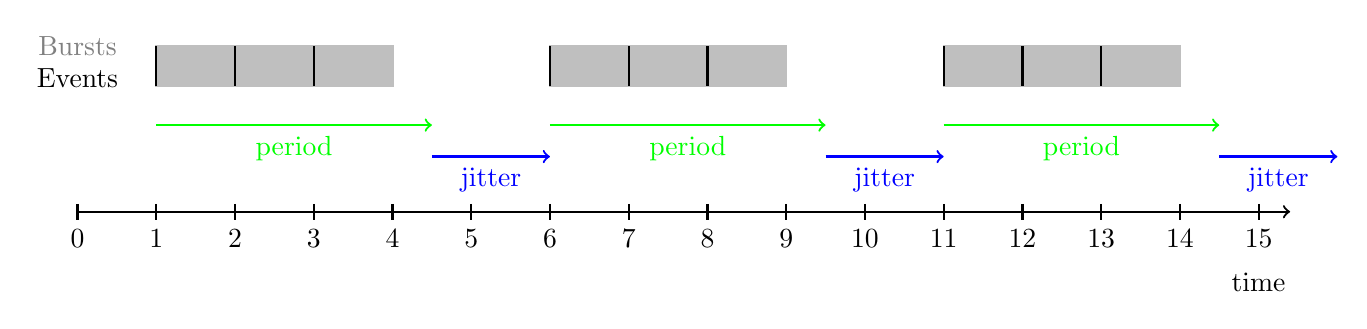
\begin{tikzpicture}[thick]
	% time axis
	\foreach \x in {0,...,15}
	\draw (\x,-4) -- (\x,-4.2) node[anchor=north] {\x};
	\draw[->] (0, -4.1) -- (15.4, -4.1);
	\node at(15, -5) {time};
	
	% bursts
	\node[gray] at (0, -2){Bursts};
	\draw [fill=lightgray, lightgray] (1, -2) rectangle (4,-2.5);
	\draw [fill=lightgray, lightgray] (6, -2) rectangle (9,-2.5);
	\draw [fill=lightgray, lightgray] (11, -2) rectangle (14,-2.5);
%	\draw [fill=lightgray, lightgray] (16, -2) rectangle (19,-2.5);
	% events
	\node at (0, -2.4){Events};
	%\node at (0, -2.15){events};
	\foreach \x in {1, 6, 11}
	{
		% events
		\draw[-] (\x, -2) -- (\x, -2.5);
		\draw[-] (\x+1, -2) -- (\x+1, -2.5);
		\draw[-] (\x+2, -2) -- (\x+2, -2.5);
		% periods
		\draw[->, green] (\x, -3) -- (\x+3.5, -3);
		\node[green] at (\x+1.75, -3.3){period};
		%jitters
		\draw[->, blue] (\x+3.5,-3.4) -- (\x+5, -3.4);
		\node[blue] at (\x+4.25, -3.7) {jitter};
	}
	\end{tikzpicture}
	\caption{BurstPatternEventTriggering \textit{patternPeriod} and \textit{patternJitter} \textbf{accumulating}}
	\label{fig:BurstPatternEventTriggering1}
\end{figure}
\begin{figure}
	\centering
	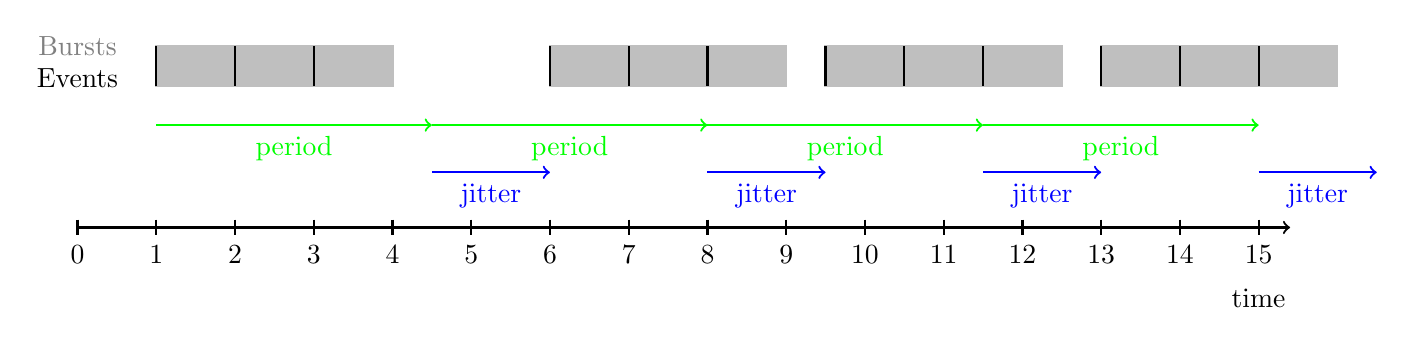
\begin{tikzpicture}[thick]
	% time axis
	\foreach \x in {0,...,15}
	\draw (\x,-4.2) -- (\x,-4.4) node[anchor=north] {\x};
	\draw[->] (0, -4.3) -- (15.4, -4.3);
	\node at(15, -5.2) {time};
	
	% bursts
	\node[gray] at (0, -2){Bursts};
	\draw [fill=lightgray, lightgray] (1, -2) rectangle (4,-2.5);
	\node at (0, -2.4){Events};
	
	%period 1
	\draw[->, green] (1, -3) -- (4.5, -3);
	\node[green] at (2.75, -3.3){period};
	
	% jitter 1
	\draw[->, blue] (4.5,-3.6) -- (6, -3.6);
	\node[blue] at (5.25, -3.9) {jitter};
	
	\foreach \y in {0, 1, 2}
	\draw[-] (1+\y, -2) -- (1+\y, -2.5);
	\foreach \x in {4.5, 8, 11.5}{
		%bursts	
		\draw [fill=lightgray, lightgray] (\x+1.5, -2) rectangle (\x+4.5,-2.5);
		% events
		\foreach \y in {0, 1, 2}
			\draw[-] (\x+\y+1.5, -2) -- (\x+\y+1.5, -2.5);
			
	}
	\foreach \x in {4.5, 8, 11.5}
	{
		% periods
		\draw[->, green] (\x, -3) -- (\x+3.5, -3);
		\node[green] at (\x+1.75, -3.3){period};
		% jitters
		\draw[->, blue] (\x+3.5,-3.6) -- (\x+5, -3.6);
		\node[blue] at (\x+4.25, -3.9) {jitter};
		
	}

	
	\end{tikzpicture}
	\caption{BurstPatternEventTriggering \textit{patternPeriod} and \textit{patternJitter} \textbf{non-accumulating}}
	\label{fig:BurstPatternEventTriggering2}
\end{figure}

The combination of $patternPeriod$ and $patternJitter$ can be interpreted in an accumulating way, as seen in \ref{fig:BurstPatternEventTriggering1}, or in a non-accumulating way, as seen in \ref{fig:BurstPatternEventTriggering2}. In the accumulating interpretation, the reference for the periodic occurrences is only the start point of the previous burst. In the non-accumulating way, there is an global reference point for the periodic repetitions.

With the definition of $patternPeriod$ (''time distance between the beginnings of subsequent repetitions of the given burst pattern''\cite{TIMEX}) you would think, that the accumulating variant is meant. Against that, the period attribute in \textit{PeriodicEventTriggering}-Constraint is defined as ''distance between subsequent occurrences of the event''\cite{TIMEX} in the text, hence it is also understandable the accumulating way, but there is the formal definition

\begin{math}
\exists t_{reference}\forall t_n: t_{reference}+(n+1)*period\leq t_n\leq t_{reference}+(n-1)*period+jitter,
\end{math}

where $t_n$ is the time of the $n$-th event and $t_{reference}$ is a reference point, from which the periodic pattern starts, so the $PeriodicEventTriggering$-Constraint is meant to be understood in the non-accumulating way. It remains unclear, in which way the $BurstPatternEventTriggering$ is meant to be understood.

Another problem of the AUTOSAR Timing Extensions is, that they were made for design purposes, monitoring them can be difficult, as a monitor may need time and memory resources, which continuously grow with every input event. This makes online monitoring unsuitable in nearly all scenarios (more on monitorability in \ref{chapter-monitorability}). As example, we will use the \textit{BurstPatternEventTriggering} again. This time we use the attributes
\begin{itemize}
	\item
	$maxNumberOfOccurrences = INT\_MAX$\textcolor{gray}{or any significant large number}
	\item
	$minNumberOfOccurrences = 1$
	\item
	$minimumInterArrivalTime = 0$
	\item
	$patternLength = 3$
	\item
	\textcolor{gray}{$patternPeriod$} \textcolor{gray}{unused}
	\item
	\textcolor{gray}{$patternJitter$} \textcolor{gray}{unused}
\end{itemize}

Figure~\ref{fig:BurstPatternEventTriggering3} shows the application of the \emph{BurstPatternEventTriggering} constraint with the given parameters on a stream with events at the timestamps 3, 3.5, 4, 4.5. The development of possible the burst clusters with ongoing time is visualized. The gray bars show the range, in which the burst cluster can lay, the black lines show, where they definitely are. In timestamp 3 with only one event so far, only one burst has to be considered and it can lay between timestamp 0 and 6, the only limitation is, that it must include timestamp 3 with the event in that point. In Timestamp 3.5, there are two events (at 3 and 3.5) so far and there are two possibilities for burst placements. The first possibility with only one burst with both events in it, and the second possibility, where the events are in different bursts. The third graphic shows the trace in timestamp 4 with three different events so far (3, 3.5, 4) and three different possibilities for burst placements to consider. One possible burst contains all three events, the second possibility has one burst with the event at timestamp 3 and one burst with the events at 3.5 and 4 and the third possibility has one Burst with the events at 3 and 3.5 and one burst with the event at 4. The possible bursts in graphic 4 are analog to the third graphic, one possibility with one burst containing all 4 events and 3 possibilities with the first burst containing the first event, the first and second event or the first, the second and the third event and the second burst containing the remaining events. Because the minimal distance between subsequent events is not specified, an arbitrary large number of events can be placed in any interval with the length $patternLenth$.\\
In this example we see that it is possible to create an unlimited number of possibilities for burst placements within one burst length, when the \textit{minimumInterArrivalTime}-attribute is 0, which results in an infeasible resource consumption, because unlimited memory and time is needed to check the constraint in following events. Therefore, online monitoring this constraint is unsuitable in most cases.

\begin{figure}
	\centering
	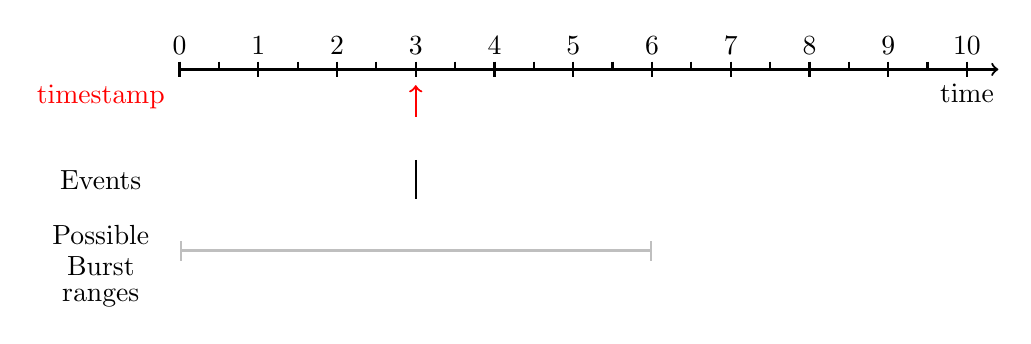
\begin{tikzpicture}[thick]
	%time axis
	\foreach \x in {0,...,10}
	{
		\draw (\x,0) -- (\x,-0.2);
		\node at (0+\x, 0.2) {\x};
	}
	\foreach \x in {0,...,9}
	\draw (\x+0.5,0) -- (\x+0.5,-0.1);
	\draw[->] (0, -0.1) -- (10.4, -0.1);
	\node at(10, -0.4) {time};
	
	\node[red] at(-1, -0.45) {timestamp};
	%watched time
	\draw[->, red] (3, -0.7)--(3, -0.3);
	
	\node at (-1, -1.5) {Events};
	\draw[-] (3, -1.25) -- (3, -1.75);
	
	\node at (-1, -2.2) {Possible};
	\node at (-1, -2.6) {Burst};
	\node at (-1, -3) {ranges};
	
	%Burst range
	\draw[|-|, lightgray] (0, -2.4) -- (6, -2.4);
	\end{tikzpicture}
	
	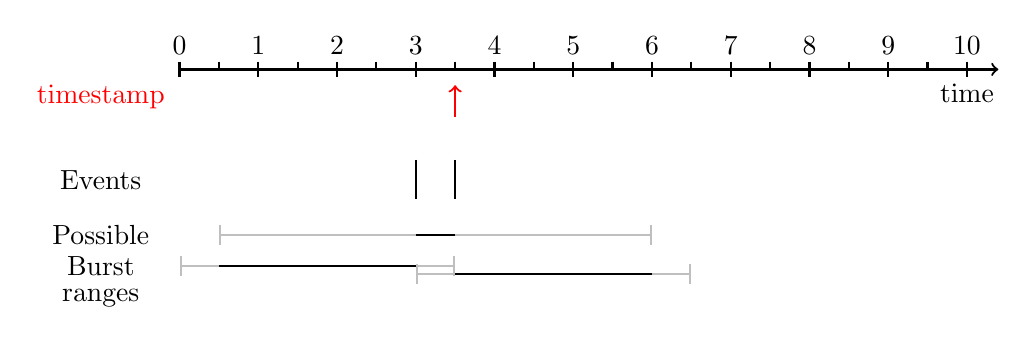
\begin{tikzpicture}[thick]
	%time axis
	\foreach \x in {0,...,10}
	{
		\draw (\x,0) -- (\x,-0.2);
		\node at (0+\x, 0.2) {\x};
	}
	\foreach \x in {0,...,9}
	\draw (\x+0.5,0) -- (\x+0.5,-0.1);
	\draw[->] (0, -0.1) -- (10.4, -0.1);
	\node at(10, -0.4) {time};
	
	\node[red] at(-1, -0.45) {timestamp};
	%watched time
	\draw[->, red] (3.5, -0.7)--(3.5, -0.3);
	
	\node at (-1, -1.5) {Events};
	\draw[-] (3, -1.25) -- (3, -1.75);
	\draw[-] (3.5, -1.25) -- (3.5, -1.75);
	
	\node at (-1, -2.2) {Possible};
	\node at (-1, -2.6) {Burst};
	\node at (-1, -3) {ranges};
	
	%Burst range 1
	\draw[|-|, lightgray] (0.5, -2.2) -- (6, -2.2);
	\draw[-] (3, -2.2) -- (3.5, -2.2);
	% Burst range 2
	\draw[|-|, lightgray] (0, -2.6) -- (3.5, -2.6);
	\draw[-] (0.5, -2.6) -- (3, -2.6);
	\draw[|-|, lightgray] (3, -2.7) -- (6.5, -2.7);
	\draw[-] (3.5, -2.7) -- (6, -2.7);
	\end{tikzpicture}
	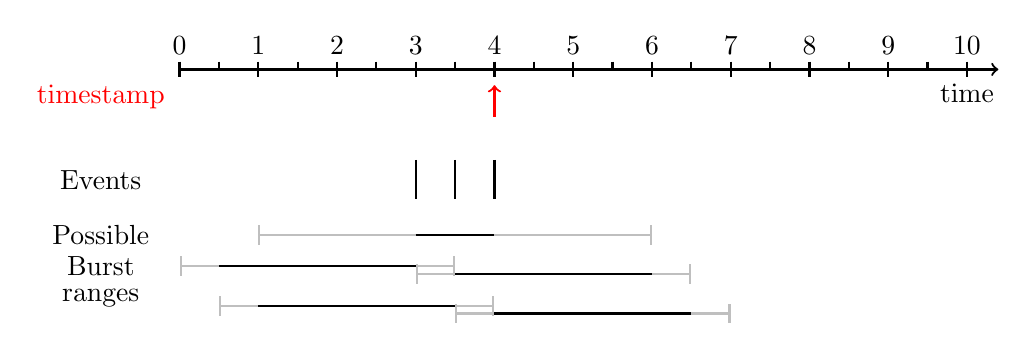
\begin{tikzpicture}[thick]
	%time axis
	\foreach \x in {0,...,10}
	{
		\draw (\x,0) -- (\x,-0.2);
		\node at (0+\x, 0.2) {\x};
	}
	\foreach \x in {0,...,9}
	\draw (\x+0.5,0) -- (\x+0.5,-0.1);
	\draw[->] (0, -0.1) -- (10.4, -0.1);
	\node at(10, -0.4) {time};
	
	\node[red] at(-1, -0.45) {timestamp};
	%watched time
	\draw[->, red] (4, -0.7)--(4, -0.3);
	
	\node at (-1, -1.5) {Events};
	\draw[-] (3, -1.25) -- (3, -1.75);
	\draw[-] (3.5, -1.25) -- (3.5, -1.75);
	\draw[-] (4, -1.25) -- (4, -1.75);
	
	\node at (-1, -2.2) {Possible};
	\node at (-1, -2.6) {Burst};
	\node at (-1, -3) {ranges};
	
	%Burst ranges poss. 1
	\draw[|-|, lightgray] (1, -2.2) -- (6, -2.2);
	\draw[-] (3, -2.2) -- (4, -2.2);
	% Burst ranges poss. 3 2.6,2.7
	\draw[|-|, lightgray] (0, -2.6) -- (3.5, -2.6);
	\draw[-] (0.5, -2.6) -- (3, -2.6);
	\draw[|-|, lightgray] (3, -2.7) -- (6.5, -2.7);
	\draw[-] (3.5, -2.7) -- (6, -2.7);
	% Burst ranges poss. 2
	\draw[|-|, lightgray] (0.5, -3.1) -- (4, -3.1);
	\draw[-] (1, -3.1) -- (3.5, -3.1);
	\draw[|-|, lightgray] (3.5, -3.2) -- (7, -3.2);
	\draw[-] (4, -3.2) -- (6.5, -3.2);
	\end{tikzpicture}
	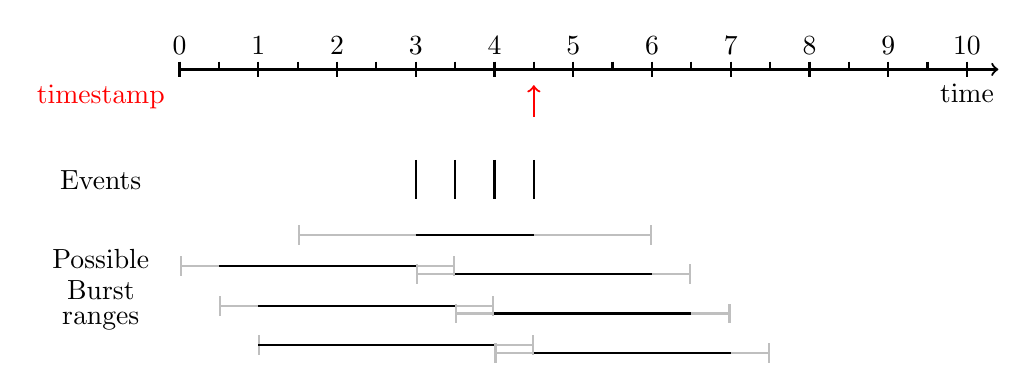
\begin{tikzpicture}[thick]
	%time axis
	\foreach \x in {0,...,10}
	{
		\draw (\x,0) -- (\x,-0.2);
		\node at (0+\x, 0.2) {\x};
	}
	\foreach \x in {0,...,9}
	\draw (\x+0.5,0) -- (\x+0.5,-0.1);
	\draw[->] (0, -0.1) -- (10.4, -0.1);
	\node at(10, -0.4) {time};
	
	\node[red] at(-1, -0.45) {timestamp};
	%watched time
	\draw[->, red] (4.5, -0.7)--(4.5, -0.3);
	
	\node at (-1, -1.5) {Events};
	\draw[-] (3, -1.25) -- (3, -1.75);
	\draw[-] (3.5, -1.25) -- (3.5, -1.75);
	\draw[-] (4, -1.25) -- (4, -1.75);
	\draw[-] (4.5, -1.25) -- (4.5, -1.75);
	
	\node at (-1, -2.5) {Possible};
	\node at (-1, -2.9) {Burst};
	\node at (-1, -3.3) {ranges};
	
	%Burst ranges poss. 1
	\draw[|-|, lightgray] (1.5, -2.2) -- (6, -2.2);
	\draw[-] (3, -2.2) -- (4.5, -2.2);
	% Burst ranges poss. 2
	\draw[|-|, lightgray] (0, -2.6) -- (3.5, -2.6);
	\draw[-] (0.5, -2.6) -- (3, -2.6);
	\draw[|-|, lightgray] (3, -2.7) -- (6.5, -2.7);
	\draw[-] (3.5, -2.7) -- (6, -2.7);
	% Burst ranges poss. 3
	\draw[|-|, lightgray] (0.5, -3.1) -- (4, -3.1);
	\draw[-] (1, -3.1) -- (3.5, -3.1);
	\draw[|-|, lightgray] (3.5, -3.2) -- (7, -3.2);
	\draw[-] (4, -3.2) -- (6.5, -3.2);
	% Burst ranges poss. 4
	\draw[|-|, lightgray] (1, -3.6) -- (4.5, -3.6);
	\draw[-] (1, -3.6) -- (4, -3.6);
	\draw[|-|, lightgray] (4, -3.7) -- (7.5, -3.7);
	\draw[-] (4.5, -3.7) -- (7, -3.7);
	\end{tikzpicture}
	\caption{BurstPatternEventTriggering Possible bursts, \textcolor{red}{$\uparrow$} shows the current time}
	\label{fig:BurstPatternEventTriggering3}
	
%TODO weiteres Beispiel für unsaubere Definition von AUTOSAR-> falsches Beispiel für file:///home/hendrik/Documents/Uni/Semester8/Quellen%20Bachelorarbeit/AutoSar%20TimEx/MethodologyAndTemplates/AUTOSAR_TPS_TimingExtensions.pdf
\end{figure}

\newpage

\section{Timing Augmented Description Language}
	As timing extension to EAST-ADL(\textbf{E}lectronics \textbf{A}rchitecture and \textbf{S}oftware \textbf{T}echnology-\textbf{A}rchitecture \textbf{D}escription \textbf{L}anguage), the TIMMO (\textbf{Tim}ing \textbf{Mo}del) project, and its successor TIMMO2USE, were initiated. A part of this project was the \textbf{T}iming \textbf{A}ugmented \textbf{D}escription \textbf{L}anguage V2 (TADL2), were created. TADL2 has similar goals as the AUTOSAR Timing Extensions, but the definitions are written in a more formalized fashion. The definitions of the AUTOSAR Timing Extensions are only textually described often, the TADL2 definitions are defined in a more formal way, as they offer a formal definition of each constraint in the timing constraint logic TiCL \cite{TIMMO2USE}. EAST-ADL is much less used in the automotive industry, but the EAST-ADL Timing Constraints are partly compatible to the AUTOSAR Timing Extensions, as they are sub- or supersets of each other. Many of the AUTOSAR Timing Extensions can be defined via a combination of TADL2 Constraints, as explained in section~\ref{comparisonConstraints}.\\
	The timing constraints are defined on events or event chains, similar to the AUTOSAR Timing Extensions. In TADL2, all events of an event chain have a color attribute, which shows the logical connection of associated events. This attribute is defined as abstract and possibly infinite datatype. The only restriction is, that an equality test on these color values must be defined. TADL2 offers 18 timing constraints, which will briefly explained in the following.
	\begin{itemize}
		\item
			The \textbf{StrongDelayConstraint} defines the minimal and maximal time distance of the events from two event sets (\emph{source} and \emph{target}).
		\item
			The \textbf{DelayConstraint} is a less strict variant of the \textbf{StrongDelayConstraint}, because it allows additional events in \emph{target}.
		\item
			The \textbf{RepeatConstraint}, \textbf{RepetitionConstraint}, \textbf{PeriodicConstraint}, \textbf{SporadicConstraint} and \textbf{ArbitraryConstraint} are describing the time distance between subsequent events, whereby they are having small semantic differences. An exact distinction between these constraints will be given in section~\ref{tadl2Constraints}.
		\item
			The \textbf{SynchronizationConstraint} and \textbf{StrongSynchronizationConstraint} define groups of event sets, whose events occur in common time intervals. The SynchronizationConstraint allows more than one event of each group per interval, the StrongSynchronizationConstraint does not.
		\item
			The \textbf{ExecutionTimeConstraint} is used to set a minimum and a maximum for the runtime of a task, not counting interruptions in the execution.
		\item
			The \textbf{OrderConstraint} defines that the $n^{th}$ event of one event set must occur before or at the $n^{th}$ event of a second event set.
		\item
			The \textbf{ComparisonConstraint} is used to describe ordering relations of timestamps.
		\item
			The \textbf{PatternConstraint} defines the time distance between periodic points in time and several events.
		\item
			The \textbf{BurstConstraint} regulates the maximum number of events in time intervals of a specific length.
		\item
			The \textbf{ReactionConstraint} describes the minimal and maximal time a response event must occur after the associated stimulus event. Additional response events are allowed, additional stimulus events not.
		\item
			The \textbf{AgeConstraint} is similar to the ReactionConstraint, but it is defined the other way around. Therefore, it describes the minimal and maximal time a stimulus event must occur before the associated response event.  Additional stimulus events are allowed, additional response events not.
		\item
			The \textbf{OutputSynchronizationConstraint} is used to describe groups of event chains, which all have the same response events. The response events of the event chain must occur in common time intervals, like in the SynchronizationConstraint. In the \textbf{InputSynchronizationConstraint}, the roles of the stimulus and response events are swapped.			
	\end{itemize}
	
\subsection{Parenthesis - Simple and Flexible Timing Constraint Logic}
	The formal definition of the TADL2 timing constraint are written in \emph{Timing Constraint Logic} (short: \emph{TiCL}), which was developed as part of the TIMMO-2-USE project. TiCL was formally introduced in \cite{TiCL}, for better understanding the key aspects of this paper will be explained in the following.\\
	The main goal of TiCL is to be formal and expandable and offering the possibility of defining finite and infinite behaviors of events. In TiCL, only points in time, when events occur, are considered, therefore every event only consists of a real number as timestamp, without the possibility of adding a data value. There are 7 syntactic categories in TiCL
	\begin{align*}
		\mathbb{R} &\text{(arithmetic constants)}\\
		Avar &\text{(arithmetic variables)}\\
		AExp &\text{(arithmetic expressions)}\\[10pt]
		%\vspace{1cm}
		Svar &\text{(set variables)}\\
		SExp &\text{(set expressions)}\\[10pt]
		%\vspace{1cm}
		TVar &\text{(time variables)}\\
		CExp &\text{(constraint expressions)}
	\end{align*}
	Arithmetic expressions can be defined as arithmetic constants, as arithmetic variables, as application of $+,-,*,/$ on arithmetic expressions, as application of the cardinality operator on a set ($|E|$, $E\in SExp$) or as measure $\lambda(E)$ ($E\in SExp$). $\lambda(E)$ is defined as Lebesgue measure, which is figuratively speaking, the length of all continuous intervals of $E$. In figure~\ref{fig:TiCLMeasureExample} an example of the measure operator $\lambda$ is visualized. The set $E$ contains all Events between the timestamps $1$ and $9$, the set $F$ contains the events at the timestamps between 2 and 4 and 6 and 7, therefore $E\setminus F$ contains the events at the timestamps $\{1, 1.5, 4.5, 5, 5.5, 7.5, 8, 8.5, 9\}$.
	$E$ consists of one continuous interval from timestamp 1 to 9 with the length of 8, $F$ consists of two continuous intervals from 2 to 4 with the length of 2 and from 6 to 7 with the length of 1, therefore $\lambda(F)=3$. $E\setminus F$ consists of three continuous intervals, the first from 1 to 1.5 (length = 0.5), the second from 4.5 to 5.5 (length = 1) and the last from 7.5 to 9 (length = 1.5). Consequently the total length of the continuous intervals of $E\setminus F$ is 3.\\
	% TODO richtig? vgl. executionTimeConstraint-> ja richtig. [x..y] beschreibt Interval mit allen mögl. Zeitpunkten dadrin.
	\begin{figure}
		\centering
		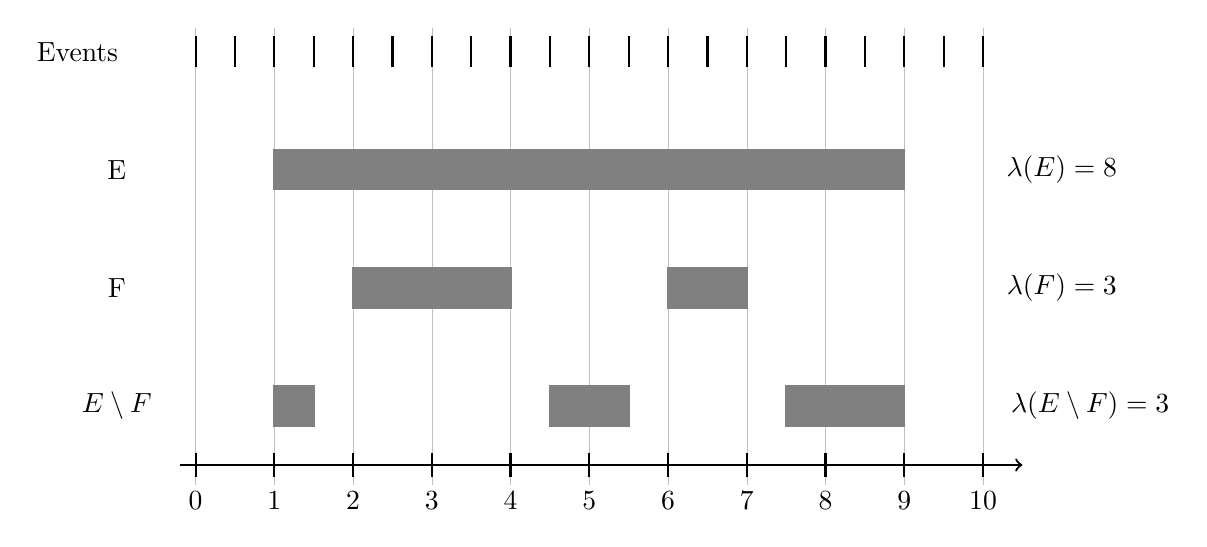
\begin{tikzpicture}[thick]
			\foreach \x in {0,...,10}
			{
				\draw[very thin, lightgray](\x, 1.8) -- (\x, -4);
				
				\draw (\x,-3.6) -- (\x,-3.9);
				\node at (0+\x, -4.2) {\x};
			}
			\draw[->] (-0.2, -3.75) -- (10.5, -3.75);
			
			\node at (-1,  0) {E};
			\draw [fill=gray,gray] (1,0.25) rectangle (9,-0.25); 
			
			\node at (-1, -1.5) {F};
			\draw [fill=gray,gray] (2,-1.25) rectangle (4,-1.75); 
			\draw [fill=gray,gray] (6,-1.25) rectangle (7,-1.75);
			
			\node at (-1, -3) {$E \setminus F$};
			\draw [fill=gray,gray] (1,-2.75) rectangle (1.5,-3.25); 
			\draw [fill=gray,gray] (4.5,-2.75) rectangle (5.5,-3.25);
			\draw [fill=gray,gray] (7.5,-2.75) rectangle (9,-3.25);
			
			\node at (11, 0) {$\lambda(E) = 8$};
			\node at (11, -1.5) {$\lambda(F) = 3$};
			\node at (11.36, -3) {$\lambda(E\setminus F) = 3$};
			
			\node at (-1.5, 1.5){Events};
			\foreach \x in {0, 0.5, ...,10}
			\draw (\x, 1.7) -- (\x, 1.3);
		\end{tikzpicture}
		\caption{Graphical example of $\lambda(E), \lambda(F)$ and $\lambda(E\setminus F)$}
		\label{fig:TiCLMeasureExample}
	\end{figure}
	Set expressions can be defined as set variables, or as set of time variables that fulfill a given constraint expression.\\
	Constraint expressions can be defined as application of the $\leq$ operator on time or arithmetic expressions, the $\in$ operator on time variables and set expressions, the logical conjunction ($\land$) on constraint expressions, the negation of constraint expressions and the $\forall$-Quantifier on arithmetic, set and time variables over a constraint expression.\\
	As extension to this definition, well known syntactic abbreviations like $true\equiv 0\leq 1$ or the $\exists$-quantifier will be used, but there are also some TiCL-specific syntactic abbreviations, like interval constructors, which will be defined and explained in the following.\\ \\
	Let $x, y\in Tvar$ and $E, F\in SExp$.\\ \\
	The interval constructor $[x<]$($[x\leq]$) is defined as $\{y: x < y\}$($\{y: x \leq y\}$), therefore the interval contains all points in time laying behind of $x$ (including $x$).\\ \\
	$[\leq x]$($[< x]$) is defined as complement of $[x<]$($[x\leq]$) and contains all timestamps laying before $x$.\\ \\
	$[x..y]$ is defined as $[x\leq]\cap[<y]$, so all points of time after $x$ and before $y$, including $x$ but not $y$, are part of this interval.\\ \\
	$[E \leq]$ is defined as $\{y : \exists x \in E : x \leq y\}$, this interval contains all points in time at and after the first timestamp in $E$.\\ \\
	$[E<]$ is equal to $\{y : \forall x \in E : x < y\}$, therefore it defines the interval containing all timestamps after the latest point of time in $E$. Please note the use of $\forall$ instead $\exists$ in the definition.\\ \\
	$[\leq E]$ ($[< E]$) is defined as $[E<]^C$ ($[E\leq]^C$), analogous to the operators on time variables.\\ \\
	$[E]$ is equal to $[E\leq]\cap[\leq E]$. It defines the time interval between the first and last element of $E$, including these points in time.\\ \\
	$E_{x<}$($E_{<x}$) is defined as $E\cap [x<]$($E\cap [<x]$). This operators filters the timestamps in $E$ so that only the points in time before (after) $x$ remain.\\ \\
	$[x..E]$ equals $[x\leq]\cap[<(E_{x<})]$. The interval begins at $x$ and ends right before the first element of $E$ after $x$.\\ \\
	$[E..F]$ is defined as $\{x:\exists y\in E:x\in[y..F]\}$ and describes the intervals, where the previous operator is applied on every element of $E$.\\ \\
	$E(i)$ is $i^{th}$ timestamp in $E$, starting by zero.\\ \\
	$E\leq F$ describes, that $E$ is a sub sequence of $F$, which means that between the earliest and latest element in $E$ all elements of $F$ are in $E$.
	

	% TODO x-y/y-x ???
	% TODO X\leq Y -> X is subsequence of Y needed???
\subsection{TADL2-Timing Constraints}
	\label{tadl2Constraints}
	For better understanding of the following chapters, the TADL Constraints will be presented next. As abbreviation and unification, all timing expressions are defined as set $\mathbb{T}$, which are understood as real numbers but expanded with $\infty$ and $-\infty$ in this chapter, but other value ranges for time expressions are possible and will be used in other parts of this thesis.\\
	We define an event as a time value, possibly combined with a data value. The range of the data values are arbitrary, infinite data types are possible as well as empty data types, when only the point in time is relevant for the constraint. All TADL constraints are defined with attributes, which can be events, timing or arithmetic expressions or sets of them. Also, \emph{EventChains} can be used as attributes. An \emph{EventChain} consists of two sets of events (\emph{stimulus} and \emph{response}),  which are causally related. All events in an \emph{EventChain} must have a color value in their data field. This color possibly has an infinite type and an equality check on the datatype of the color must be defined. It is used to check, which events of an \emph{EventChain} are directly related.
	\subsubsection{DelayConstraint}
		The \emph{DelayConstraint} has 4 attributes
		\begin{align*}
			\emph{source} & \hspace{.5cm}\text{event set}\\
			\emph{target} & \hspace{.5cm}\text{event set}\\
			\emph{lower}  & \hspace{.5cm}\text{$\mathbb{T}$ (time expression)}\\
			\emph{upper}  & \hspace{.5cm}\text{$\mathbb{T}$}
		\end{align*}
		and is defined as\\[10pt]
		\begin{math}
			DelayConstraint ( source, target, lower, upper )\\
			\Leftrightarrow \forall x\in source:\exists y\in target: lower\leq y-x\leq upper.
		\end{math}\\[10pt]
		For all events $x$ in \emph{source}, there must be an event $y$ in \emph{target}, so that the time distance between $x$ and $y$ is between \emph{lower} and \emph{upper}. Note, that \emph{lower} and \emph{upper} can have negative values and that additional events in \emph{target}, without an associated \emph{source} event are allowed.\\
		Figure~\ref{fig:delayConstraintExample} shows a visualized example of the \emph{DelayConstraint} with the attributes $lower=2$, $upper=3$, $source=\{1, 5, 6\}$ and $target=\{2, 3.5, 5, 7, 8.2, 9\}$. The first element of source at timestamp 1 results in a required event in target between the timestamp 3 and 4 that is fulfilled by the event at 3.5. The second event of source requires an target event between 7 and 8, fulfilled by the event at 7. The last event of source is satisfied by the target event at 8.2 and 9.
		\begin{figure}
			\centering
			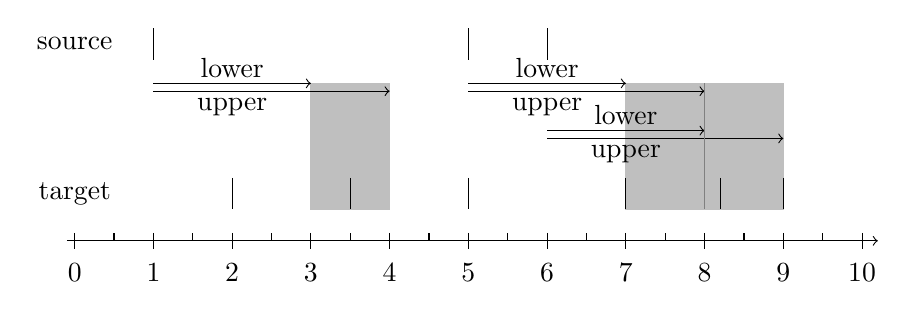
\begin{tikzpicture}
				% source events
				\node[] at (0,-0.2){source};
				\draw (1, 0) -- (1, -0.4);
				\draw (5, 0) -- (5, -0.4);
				\draw (6, 0) -- (6, -0.4);
				
				% upper/lower 1
				\draw [fill=lightgray, lightgray] (3, -0.7) rectangle (4,-2.3);
				\node at (2, -0.5){lower};
				\node at (2, -1){upper};
				\draw[->] (1,-0.7) -- (3, -0.7);
				\draw[->] (1, -0.8) -- (4, -0.8);
				
				
				% upper/lower 2
				\draw [fill=lightgray, lightgray] (7, -0.7) rectangle (8,-2.3);
				\node at (6, -0.5){lower};
				\node at (6, -1){upper};
				\draw[->] (5,-0.7) -- (7, -0.7);
				\draw[->] (5, -0.8) -- (8, -0.8);
				
				% upper/lower 3
				\draw [fill=lightgray, lightgray] (8, -0.7) rectangle (9,-2.3);
				\node at (7, -1.1){lower};
				\node at (7, -1.6){upper};
				\draw[->] (6,-1.3) -- (8, -1.3);
				\draw[->] (6, -1.4) -- (9, -1.4);
				% target events
				\node[] at (0,-2.1){target};
				\draw (2, -1.9) -- (2, -2.3);
				\draw (3.5, -1.9) -- (3.5, -2.3);
				\draw (5, -1.9) -- (5, -2.3);
				\draw (7, -1.9) -- (7, -2.3);
				\draw (8.2, -1.9) -- (8.2, -2.3);
				\draw (9, -1.9) -- (9, -2.3);
				
				\foreach \x in {0, 1, ..., 10}{
					\draw (\x, -2.6) -- (\x, -2.8);
					\node at(\x, -3.1) {\x};
				}
			
				\foreach \x in {0.5, 1.5, ..., 9.5}{
					\draw (\x, -2.7) -- (\x, -2.6);
				}
				\draw[->] (-0.1, -2.7) -- (10.2, -2.7);
				
				\draw[gray] (8,-0.7)--(8,-2.3);
					
			\end{tikzpicture}
			\caption{Example DelayConstraint - $lower = 2$, $upper = 3$}
			\label{fig:delayConstraintExample}
		\end{figure}
	\subsubsection{StrongDelayConstraint}
		The \emph{StrongDelayConstraint} has 4 attributes
		\begin{align*}
			\emph{source} & \hspace{.5cm}\text{event set}\\
			\emph{target} & \hspace{.5cm}\text{event set}\\
			\emph{lower}  & \hspace{.5cm}\text{$\mathbb{T}$}\\
			\emph{upper}  & \hspace{.5cm}\text{$\mathbb{T}$}
		\end{align*}
		and is defined as\\[10pt]
		\begin{math}
			StrongDelayConstraint( source, target, lower, upper )\\
			|source| = |target| \land\\
			\forall i: \forall x: x=source(i) \Rightarrow \exists y: y=target(i)\land lower\leq y-x\leq upper.
		\end{math}\\[10pt]
		The \emph{StrongDelayConstraint} is a stricter version of the \emph{DelayConstraint}, as it requires a bijective assignment between the source and target events, therefore additional events in target without matching source event are not allowed. Figure~\ref{fig:StrongDelayConstraintExample} shows an example of the \emph{StrongDelayConstraint}. The example is the same as in the previous constraint, but without the additional target events at 2, 5 and 8.2.
 		\begin{figure}
			\centering
		 	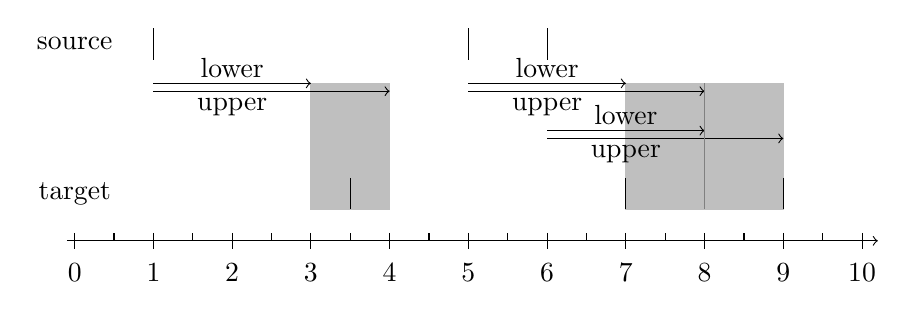
\begin{tikzpicture}
		 	% source events
		 	\node[] at (0,-0.2){source};
		 	\draw (1, 0) -- (1, -0.4);
		 	\draw (5, 0) -- (5, -0.4);
		 	\draw (6, 0) -- (6, -0.4);
		 	
		 	% upper/lower 1
		 	\draw [fill=lightgray, lightgray] (3, -0.7) rectangle (4,-2.3);
		 	\node at (2, -0.5){lower};
		 	\node at (2, -1){upper};
		 	\draw[->] (1,-0.7) -- (3, -0.7);
		 	\draw[->] (1, -0.8) -- (4, -0.8);
		 	
		 	
		 	% upper/lower 2
		 	\draw [fill=lightgray, lightgray] (7, -0.7) rectangle (8,-2.3);
		 	\node at (6, -0.5){lower};
		 	\node at (6, -1){upper};
		 	\draw[->] (5,-0.7) -- (7, -0.7);
		 	\draw[->] (5, -0.8) -- (8, -0.8);
		 	
		 	% upper/lower 3
		 	\draw [fill=lightgray, lightgray] (8, -0.7) rectangle (9,-2.3);
		 	\node at (7, -1.1){lower};
		 	\node at (7, -1.6){upper};
		 	\draw[->] (6,-1.3) -- (8, -1.3);
		 	\draw[->] (6, -1.4) -- (9, -1.4);
		 	% target events
		 	\node[] at (0,-2.1){target};
		 	\draw (3.5, -1.9) -- (3.5, -2.3);
		 	\draw (7, -1.9) -- (7, -2.3);
		 	\draw (9, -1.9) -- (9, -2.3);
		 	
			\foreach \x in {0, 1, ..., 10}{
				\draw (\x, -2.6) -- (\x, -2.8);
				\node at(\x, -3.1) {\x};
			}
		
			\foreach \x in {0.5, 1.5, ..., 9.5}{
				\draw (\x, -2.7) -- (\x, -2.6);
			}
			\draw[->] (-0.1, -2.7) -- (10.2, -2.7);
		 	
		 	\draw[gray] (8,-0.7)--(8,-2.3);
		 	\end{tikzpicture}
		 	\caption{Example StrongDelayConstraint - $lower = 2$, $upper = 3$}
		 	\label{fig:StrongDelayConstraintExample}
		 \end{figure}
	\subsubsection{RepeatConstraint}
		The \emph{RepeatConstraint} also has 4 attributes
		\begin{align*}
			\emph{event} & \hspace{.5cm}\text{event set}\\
			\emph{lower} & \hspace{.5cm}\text{$\mathbb{T}$}\\
			\emph{upper} & \hspace{.5cm}\text{$\mathbb{T}$}\\
			\emph{span}	 & \hspace{.5cm}\text{$integer$}\\
		\end{align*}
		and is defined as\\[10pt]
		\begin{math}
			RepeatConstraint ( event, lower, upper, span )\\
			\Leftrightarrow\forall X\leq event: |X|=span+1\Rightarrow lower \leq \lambda([X])\leq upper.
		\end{math}\\[10pt]
		As reminder, the $\leq$-operator over two sets of events $A, B$ describes, that $A$ is a sub sequence of $B$, the $\lambda(A)$-function calculates the total length of all continuous intervals in $A$ and $[A]$ is the time interval between the oldest and newest event in $A$.\\ \\
		The definition of the \textit{RepeatConstraint} specifies that the length of each time interval containing $span+1$ subsequent events must be between $upper$ and $lower$.\\
		The idea behind this constraint is to define repeated occurrences of events, with the possibility of overlapping, specified by the \emph{span} attribute. After any event $x$, there are $span-1$ events and then the next event must be between $lower$ and $upper$ after $x$.\\
		Figure~\ref{fig:RepeatConstraintExample1} shows an example of the RepeatConstraint with the attributes $event=\{3,5,8,...\}$, $lower=upper=2$ and $span=1$. Because $lower$ is equal to $upper$ and $span$ is 1, the events are following a strictly periodic pattern after the first event. Figure~\ref{fig:RepeatConstraintExample2} shows a more complex example with events at $\{0, 2, 4, 7, 9, 11,...\}$, $lower=4$, $upper=5$ and $span=2$. The $span$-attribute is 2, so the time distances between all subsequent events with an even index are considered, as well as the distances between subsequent events with an uneven index. 
		
		\begin{figure}
			\centering
			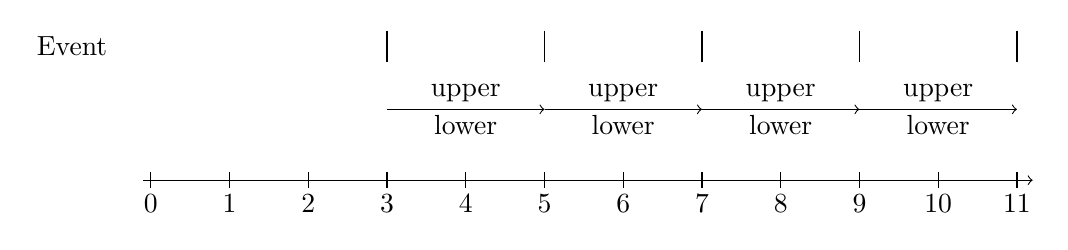
\begin{tikzpicture}
				% events
				\node at(-1 , 0.2){Event}; 
				\foreach \x in {3,5,...,9}{
					\draw (\x, 0.4) -- (\x, 0);
					\draw[->] (\x, -0.6) -- (\x+2, -0.6);
					\node at(\x+1, -0.8){lower};
					\node at(\x+1, -0.4){upper};
				}
				\draw (11, 0.4) -- (11, 0);
				% time axis
				\foreach \x in {0,...,11}{
					\draw (\x, -1.4) -- (\x, -1.6);
					\node at(\x, -1.8){\x};
				}
				\draw[->] (-0.1, -1.5) -- (11.2, -1.5);
			\end{tikzpicture}
			\caption{Example RepeatConstraint - $lower = 2$, $upper = 2$, $span = 1$}
			\label{fig:RepeatConstraintExample1}
		\end{figure}
		\begin{figure}
			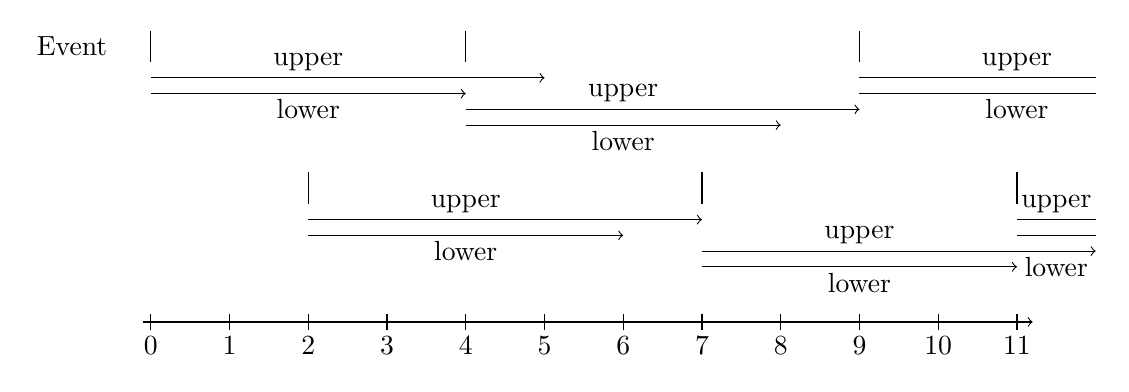
\begin{tikzpicture}
				\node at(-1, 0.2){Event};
				%eventreihe 1
				\foreach \x in {0, 4, 9} {
					\draw (\x,0) -- (\x, 0.4);
				}
				\foreach \x in {0} {
					\node at (\x+2, 0) {upper};
					\draw[->] (\x, -0.2) -- (\x+5, -0.2);
					\draw[->] (\x, -0.4) -- (\x+4, -0.4);
					\node at (\x+2, -0.6) {lower};
				}
				\foreach \x in {9} {
					\node at (\x+2, 0) {upper};
					\draw[-] (\x, -0.2) -- (12, -0.2);
					\draw[-] (\x, -0.4) -- (12, -0.4);
					\node at (\x+2, -0.6) {lower};
				}
				\foreach \x in {4} {
					\node at (\x+2, -0.4) {upper};
					\draw[->] (\x, -0.6) -- (\x+5, -0.6);
					\draw[->] (\x, -0.8) -- (\x+4, -0.8);
					\node at (\x+2, -1) {lower};
				}
				%eventreihe 2
				\foreach \x in {2, 7, 11} {
					\draw (\x,-1.4) -- (\x, -1.8);
				}
				\foreach \x in {2} {
					\node at (\x+2, -1.8) {upper};
					\draw[->] (\x, -2) -- (\x+5, -2);
					\draw[->] (\x, -2.2) -- (\x+4, -2.2);
					\node at (\x+2, -2.4) {lower};
				}
				\foreach \x in {11} {
					\node at (\x+0.5, -1.8) {upper};
					\draw[-] (\x, -2) -- (12, -2);
					\draw[-] (\x, -2.2) -- (12, -2.2);
					\node at (\x+0.5, -2.6) {lower};
				}
				\foreach \x in {7} {
					\node at (\x+2, -2.2) {upper};
					\draw[->] (\x, -2.4) -- (\x+5, -2.4);
					\draw[->] (\x, -2.6) -- (\x+4, -2.6);
					\node at (\x+2, -2.8) {lower};
				}
				%time axis
				\foreach \y in {-3.2}{
					\foreach \x in {0,...,11}{
						\draw (\x, \y) -- (\x, \y-0.2);
						\node at(\x, \y-0.4){\x};
					}
					\draw[->] (-0.1, \y-0.1) -- (11.2, \y-0.1);
				}
			\end{tikzpicture}
			\caption{Example RepeatConstraint - $lower = 4$, $upper = 5$, $span = 2$}
			\label{fig:RepeatConstraintExample2}
		\end{figure}
	
	\subsubsection{RepetitionConstraint}
		The \emph{RepetitionConstraint} has 5 attributes
		\begin{align*}
			\emph{event} & \hspace{.5cm}\text{event set}\\
			\emph{lower} & \hspace{.5cm}\text{$\mathbb{T}$}\\
			\emph{upper} & \hspace{.5cm}\text{$\mathbb{T}$}\\
			\emph{span}	 & \hspace{.5cm}\text{$integer$}\\
			\emph{jitter}& \hspace{.5cm}\mathbb{T}
		\end{align*}
		and is defined via the \emph{RepeatConstraint} and the \emph{StrongDelayConstraint} as\\[10pt]
		\begin{math}
			RepetitionConstraint ( event, lower, upper, span, jitter )\\
			\Leftrightarrow
			\exists X: RepeatConstraint(X, lower, upper, span) \land \\
			\text{\hspace{1cm}}StrongDelayConstraint(X, event, 0, jitter)
		\end{math}\\[10pt]
		where $X$ is a set of arbitrary time stamps, that follow the structure of the \emph{RepeatConstraint}(various(\emph{span}) loose periodic repetitions). The actual points in time of \emph{event} lay between the timestamps of $X$ and $jitter$ after that. For each point of time there is exactly one, corresponding timestamp in $X$.
		Figure~\ref{fig:RepetitionConstraintExample} shows an example of the \emph{RepetitionConstraint} with the attributes $event=\{0.5, 3.3, 4.7, 7.6, 9.9, ...\}$, $lower=4$, $upper=5$, $span=2$ and $jitter=1$. The shown timestamps of $X$ are only one possibility and may change due to later elements of $event$.
		
		\begin{figure}
			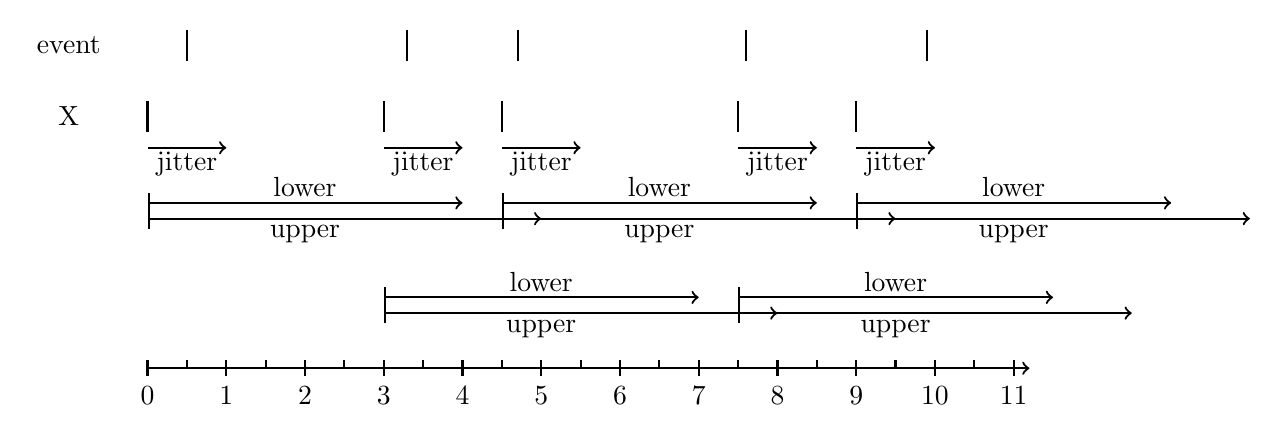
\begin{tikzpicture}[thick]
				% time axis
				\foreach \y in {-4}{
					\foreach \x in {0,...,11}
					\draw (\x,\y) -- (\x,\y-0.2) node[anchor=north] {\x};
					\foreach \x in {0.5,1.5,...,10.5}
					\draw (\x,\y) -- (\x,\y-0.1);
					\draw[->] (0,\y-0.1) -- (11.2, \y-0.1);
				}
			\node[] at (-1, 0) {event};
			\foreach \x in {0.5, 3.3, 4.7, 7.6, 9.9}
				\draw (\x, 0.2) -- (\x, -0.2);
			
			\node[] at (-1, -0.9) {X};
			\foreach \x in {0, 3, 4.5, 7.5, 9}{
				\draw (\x, -0.7) -- (\x, -1.1);
				\draw[->] (\x, -1.3) -- (\x+1, -1.3);
				\node at (\x+0.5, -1.5) {jitter};
			}
			\foreach \x in {0, 4.5, 9}{
				\node at (\x+2, -1.8) {lower};
				\draw[|->] (\x, -2) -- (\x+4, -2);
				\draw[|->] (\x, -2.2) -- (\x+5, -2.2);
				\node at (\x+2, -2.4) {upper};
			}
			\foreach \x in {3, 7.5}{
				\node at (\x+2, -3) {lower};
				\draw[|->] (\x, -3.2) -- (\x+4, -3.2);
				\draw[|->] (\x, -3.4) -- (\x+5, -3.4);
				\node at (\x+2, -3.6) {upper};
			}
			\end{tikzpicture}
			\caption{Example RepetitionConstraint - $lower = 4$, $upper = 5$, $span = 2$, $jitter=1$}
			\label{fig:RepetitionConstraintExample}
		\end{figure}
		
	
	\subsubsection{SynchronizationConstraint}
		The \emph{SynchronizationConstraint} has 2 attributes
		\begin{align*}
			\emph{event} & \hspace{.5cm}\text{set of event sets, $|event|\geq 2$}\\
			\emph{tolerance} & \hspace{.5cm}\mathbb{T}
		\end{align*}
		and is defined via the \emph{DelayConstraint} as\\[10pt]
		\begin{math}
			SynchronizationConstraint ( event_1, ..., event_n, tolerance )\\
			\Leftrightarrow\exists X: \forall i: DelayConstraint(X, event_i, 0, tolerance) \land\\
			\text{\hspace{1cm}}DelayConstraint(event_i, X, -tolerance, 0)
		\end{math}\\[10pt]
		$X$ is a set of timestamps and there must be at least one timestamp in each set of \emph{event} that is between an element of $X$ and $tolerance$ after that. Also, for each element in any set of \emph{event}, there must be a matching element of $X$.\\
		In figure~\ref{fig:SynchronizationConstraintExample} is an example of the \emph{SynchronizationConstraint} with the attributes $event=\{\{0.5, 3, 7, 7.5\}, \{0.7, 2.5, 7.3, 7.8\}, \{1.2, 3.2, 3.3, 3.4, 7.6, 8.4\}\}$ and $tolerance = 1$. The first points in time of each element of event form the first cluster, the corresponding element of $X$ can be between $0.2$ and $0.5$. For simplification, only the latest possible value for the element of $X$ are shown, which is the first event of the synchronization cluster. In the second cluster of events it can be seen that multiple timestamps from one element of $event$ can be associated with a single element of $X$. The third and fourth cluster show, that overlapping is also possible.
		\begin{figure}			
			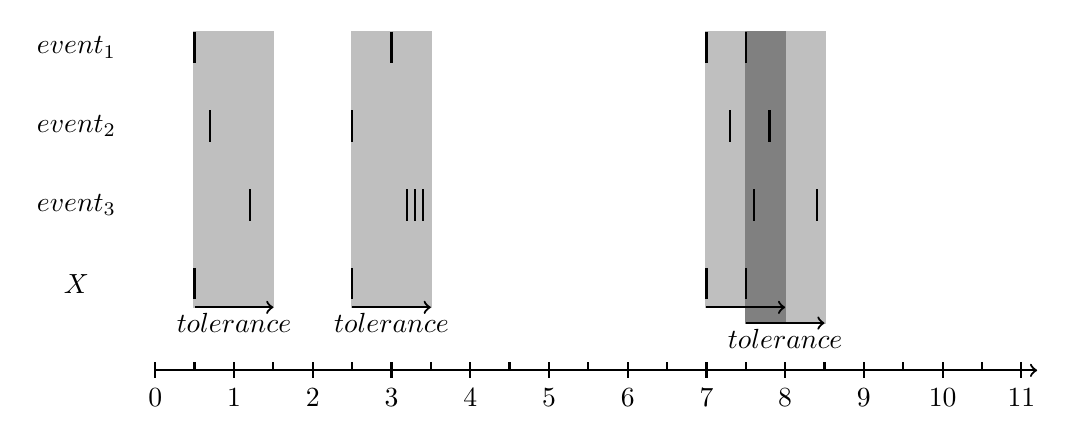
\begin{tikzpicture}[thick]
				% tolerance rectangles
				\foreach \x in {0.5, 2.5, 7}
					\draw [fill=lightgray, lightgray] (\x, 0.2) rectangle (\x+1, -3.3);
				\draw [fill=lightgray, lightgray] (7.5, 0.2) rectangle (8.5, -3.5);
				\draw [fill=gray, gray] (7.5, 0.2) rectangle (8, -3.5);
				% time axis
				\foreach \y in {-4}{
					\foreach \x in {0,...,11}
						\draw (\x,\y) -- (\x,\y-0.2) node[anchor=north] {\x};
					\foreach \x in {0.5,1.5,...,10.5}
						\draw (\x,\y) -- (\x,\y-0.1);
					\draw[->] (0,\y-0.1) -- (11.2, \y-0.1);
				}
				
				\node at (-1, 0){$event_1$};
				\foreach \x in {0.5, 3, 7, 7.5}
					\draw (\x, 0.2) -- (\x, -0.2);
				
				\node at (-1, -1){$event_2$};
				\foreach \x in {0.7, 2.5, 7.3, 7.8}
					\draw (\x, -0.8) -- (\x, -1.2);
				
				\node at (-1, -2){$event_3$};
				\foreach \x in {1.2, 3.2, 3.3, 3.4, 7.6, 8.4}
					\draw (\x, -1.8) -- (\x, -2.2);
					
				\node at (-1, -3){$X$};
				\foreach \x in {0.5, 2.5}{
					\draw (\x, -2.8) -- (\x, -3.2);
					\draw[->] (\x, -3.3) -- (\x+1, -3.3);
					\node at (\x+0.5, -3.5){$tolerance$};
				}
				\foreach \x in {7}{
					\draw (\x, -2.8) -- (\x, -3.2);
					\draw[->] (\x, -3.3) -- (\x+1, -3.3);
				}
				\foreach \x in {7.5}{
					\draw (\x, -2.8) -- (\x, -3.2);
					\draw[->] (\x, -3.5) -- (\x+1, -3.5);
					\node at (\x+0.5, -3.7){$tolerance$};
				}
					
			\end{tikzpicture}
			\caption{Example SynchronizationConstraint - $tolerance = 1$}
			\label{fig:SynchronizationConstraintExample}
		\end{figure}
		
		
		
	\subsubsection{StrongSynchronizationConstraint}
		The \emph{StrongSynchronizationConstraint} has the same two attributes as the \emph{SynchronizationConstraint}
		\begin{align*}
			\emph{event} & \hspace{.5cm}\text{set of event sets, $|event|\geq 2$}\\
			\emph{tolerance} & \hspace{.5cm}\mathbb{T}
		\end{align*}
		and is defined as\\[10pt]
		\begin{math}\\
			StrongSynchronizationConstraint ( event_1, …, event_n, tolerance )\\
			\Leftrightarrow\exists X: \forall i: StrongDelayConstraint(X, event_i, 0, tolerance)
		\end{math}\\[10pt]
		This constraint is a stricter variant of the \emph{SynchronizationConstraint}, as it requires a bijective assignment between the elements of $X$ to one element of each set of $event$. For every $x\in X$, only one corresponding timestamp per set in $event$ is allowed, like seen in figure~\ref{fig:StrongSynchronizationConstraintExample}, which shows the same example as the one for the \emph{SynchronizationConstraint}, but the excess time stamps at $3.2$ and $3.3$ have been removed.
			\begin{figure}			
				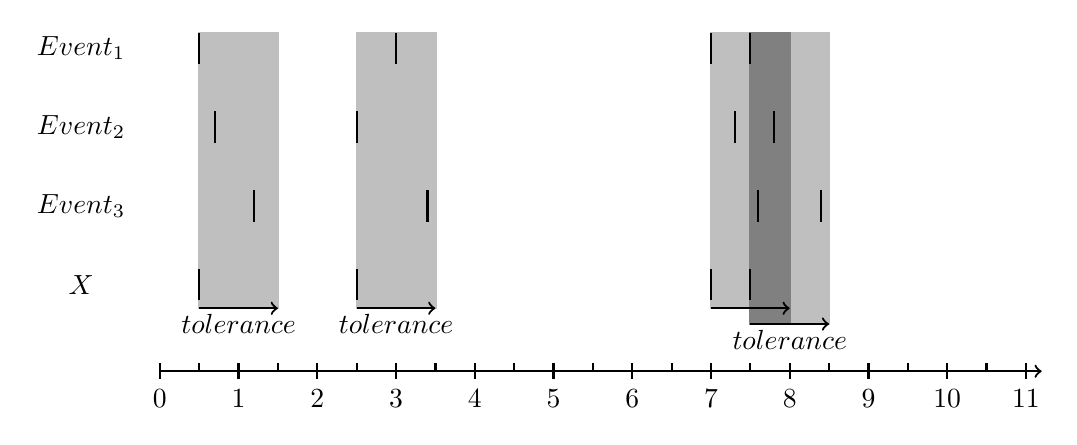
\begin{tikzpicture}[thick]
				% tolerance rectangles
				\foreach \x in {0.5, 2.5, 7}
				\draw [fill=lightgray, lightgray] (\x, 0.2) rectangle (\x+1, -3.3);
				\draw [fill=lightgray, lightgray] (7.5, 0.2) rectangle (8.5, -3.5);
				\draw [fill=gray, gray] (7.5, 0.2) rectangle (8, -3.5);
				% time axis
				\foreach \y in {-4}{
					\foreach \x in {0,...,11}
					\draw (\x,\y) -- (\x,\y-0.2) node[anchor=north] {\x};
					\foreach \x in {0.5,1.5,...,10.5}
					\draw (\x,\y) -- (\x,\y-0.1);
					\draw[->] (0,\y-0.1) -- (11.2, \y-0.1);
				}
				
				\node at (-1, 0){$Event_1$};
				\foreach \x in {0.5, 3, 7, 7.5}
				\draw (\x, 0.2) -- (\x, -0.2);
				
				\node at (-1, -1){$Event_2$};
				\foreach \x in {0.7, 2.5, 7.3, 7.8}
				\draw (\x, -0.8) -- (\x, -1.2);
				
				\node at (-1, -2){$Event_3$};
				\foreach \x in {1.2, 3.4, 7.6, 8.4}
				\draw (\x, -1.8) -- (\x, -2.2);
				
				\node at (-1, -3){$X$};
				\foreach \x in {0.5, 2.5}{
					\draw (\x, -2.8) -- (\x, -3.2);
					\draw[->] (\x, -3.3) -- (\x+1, -3.3);
					\node at (\x+0.5, -3.5){$tolerance$};
				}
				\foreach \x in {7}{
					\draw (\x, -2.8) -- (\x, -3.2);
					\draw[->] (\x, -3.3) -- (\x+1, -3.3);
				}
				\foreach \x in {7.5}{
					\draw (\x, -2.8) -- (\x, -3.2);
					\draw[->] (\x, -3.5) -- (\x+1, -3.5);
					\node at (\x+0.5, -3.7){$tolerance$};
				}
			
			\end{tikzpicture}
			\caption{Example StrongSynchronizationConstraint - $tolerance = 1$}
			\label{fig:StrongSynchronizationConstraintExample}
		\end{figure}
		
		
	\subsubsection{ExecutionTimeConstraint}
		The \emph{ExecutionTimeConstraints} takes 6 attributes
		\begin{align*}
			\emph{start} & \hspace{.5cm}\text{set of events}\\
			\emph{stop} & \hspace{.5cm}\text{set of events}\\
			\emph{preempt} & \hspace{.5cm}\text{set of events}\\
			\emph{resume} & \hspace{.5cm}\text{set of events}\\
			\emph{lower} & \hspace{.5cm}\mathbb{T}\\
			\emph{upper} & \hspace{.5cm}\mathbb{T}\\
		\end{align*}
		and is defined as\\[10pt]
		\begin{math}
			ExecutionTimeConstraint (start, stop, preempt, resume, lower, upper)\\
			\Leftrightarrow\forall x\in start: lower\leq \lambda([x..stop]\setminus[preempt..resume]) \leq upper
		\end{math}\\[10pt]
		The interval constructor $\forall x\in start: [x..stop]$ defines the time interval between each point in time of $start$ until the next element of $stop$, excluding the $stop$ timestamp. $[preempt..resume]$ defines the intervals between each element of preempt until the next timestamp of resume and is removed from the considered interval length.\\
		The Idea behind this constraint is to define the run time of a task, without counting interruptions.\\
		Figure~\ref{fig:ExecutionTimeConstraintExample} shows an example of the \emph{ExecutionTimeConstraints} with $start=\{1\}$, $end=\{7\}$, $preempt=\{2, 5\}$ and $resume = \{3, 6.5\}$. Therefore, $[start..end]$ spans the interval from time 1 to 7 with the length of 6 and $[preempt..resume]$ spans two intervals, 2 to 3 and 5 to 6.5 with the length 1 and 1.5. As result, $\lambda([x..stop]\setminus[preempt..resume])$ for $x = 1$ is 3.5 and the constraint is fulfilled, if, and only if, lower is equal or \emph{lower} than 3.5 and \emph{upper} is greater than that.\\
		\begin{figure}
   			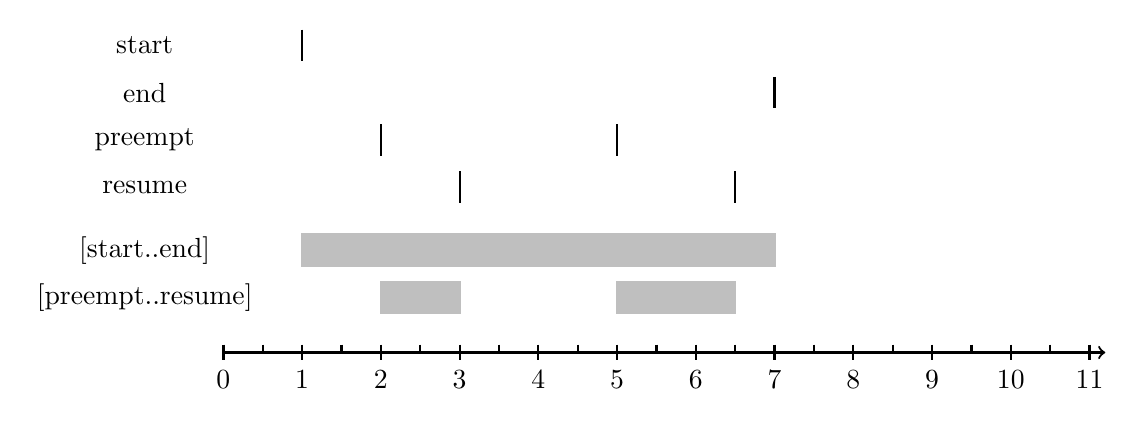
\begin{tikzpicture}[thick]
				% time axis
				\foreach \y in {-4}{
					\foreach \x in {0,...,11}
					\draw (\x,\y) -- (\x,\y-0.2) node[anchor=north] {\x};
					\foreach \x in {0.5,1.5,...,10.5}
					\draw (\x,\y) -- (\x,\y-0.1);
					\draw[->] (0,\y-0.1) -- (11.2, \y-0.1);
				}
				% start
				\node at (-1, -0.2) {start};
				\draw[] (1,0) -- (1,-0.4);
				% end
				\node at (-1, -0.8) {end};
				\draw[] (7, -0.6) -- (7, -1);
				%preempt
				\node at (-1, -1.4) {preempt};
				\draw[] (2, -1.2) -- (2, -1.6);
				\draw[] (5, -1.2) -- (5, -1.6);
				%resume
				\node at (-1, -2) {resume};
				\draw[] (3, -1.8) -- (3, -2.2);
				\draw[] (6.5, -1.8) -- (6.5, -2.2);
				
				\node at (-1, -2.8) {[start..end]};
				\draw [fill=lightgray, lightgray] (1, -2.6) rectangle (7, -3.0);
				
				\node at (-1, -3.4) {[preempt..resume]};
				\draw [fill=lightgray, lightgray] (2, -3.2) rectangle (3, -3.6);
				\draw [fill=lightgray, lightgray] (5, -3.2) rectangle (6.5, -3.6);
			\end{tikzpicture}
			\caption{Example ExecutionTimeConstraint}
			\label{fig:ExecutionTimeConstraintExample}
		\end{figure}
		
	\subsubsection{OrderConstraint}
		The \emph{OrderConstraint} takes two attributes
		\begin{align*}
			\emph{source} & \hspace{.5cm}\text{set of events}\\
			\emph{target} & \hspace{.5cm}\text{set of events}
		\end{align*}
		and is defined as\\[10pt]
		\begin{math}
			OrderConstraint ( source, target )\\
			\Leftrightarrow|source| = |target| \land \forall i:\exists x: x=source(i)\Rightarrow \exists y: y=target(i)\land < x \leq y
		\end{math}\\[10pt]
		This constraints ensures the order of events, so that the $i$-th event of $target$ occurs after the $i$-th event of $source$. Also, the number of events in \emph{source} and \emph{target} must be equal.\\
		Figure~\ref{fig:OrderConstraintExample} visualizes an example of the \emph{OrderConstraint} with $source = \{1, 4, 6, 7\}$ and $target = \{3, 5, 9, 9.5\}$. The constraint is fulfilled, because the number of elements is equal and each $i$-th timestamp in \emph{target} is later that the $i$-th timestamp of $source$.
		\begin{figure}
			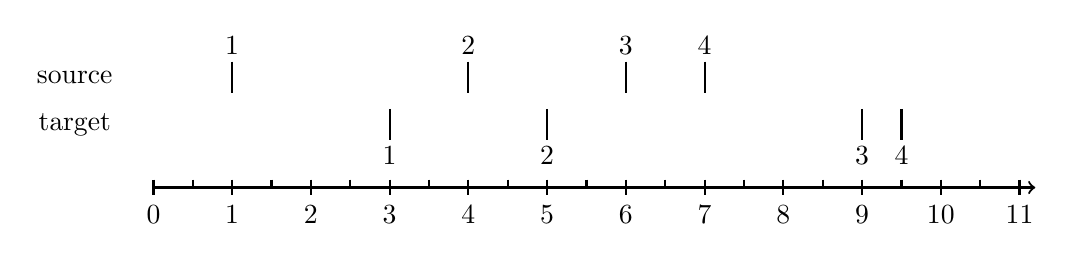
\begin{tikzpicture}[thick]
				% time axis
				\foreach \y in {-1.5}{
					\foreach \x in {0,...,11}
					\draw (\x,\y) -- (\x,\y-0.2) node[anchor=north] {\x};
					\foreach \x in {0.5,1.5,...,10.5}
					\draw (\x,\y) -- (\x,\y-0.1);
					\draw[->] (0,\y-0.1) -- (11.2, \y-0.1);
				}
				% start
				\node at (-1, -0.2) {source};
				\foreach \x in {1, 4, 6, 7}{
					\draw[] (\x,0) -- (\x,-0.4);
				}
				\node at (1, 0.2) {1};
				\node at (4, 0.2) {2};
				\node at (6, 0.2) {3};
				\node at (7, 0.2) {4};
				% end
				\node at (-1, -0.8) {target};
				\foreach \x in {3, 5, 9, 9.5}{
					\draw[] (\x,-0.6) -- (\x,-1);
				}
				\node at (3, -1.2) {1};
				\node at (5, -1.2) {2};
				\node at (9, -1.2) {3};
				\node at (9.5, -1.2) {4};
			\end{tikzpicture}
			\caption{Example OrderConstraint}
			\label{fig:OrderConstraintExample}
		\end{figure}
		
		
	\subsubsection{ComparisonConstraint}
		The \emph{ComparisonConstraint} is significant different to all previous and following constraints, as it does not describe the behavior of events and only compares two time expressions. It takes 3 attributes
		\begin{align*}
			\emph{leftOperand} 	& \hspace{.5cm}\mathbb{T}\\
			\emph{rightOperand} & \hspace{.5cm}\mathbb{T}\\
			\emph{operator}		& \hspace{.5cm} \text{comparisonOperator}(\in \{LessThanOrEqual, LessThan,\\
								& \hspace{3.5cm} GreaterThanOrEqual, GreaterThan, Equal\})
		\end{align*}
		The definition is pretty straight forward as it only applies the given operator to the operands:\\[10pt]
		\begin{math}
			ComparisonConstraint(leftOperand, rightOperand, LessThanOrEqual)\\
				\Leftrightarrow leftOperand \leq rightOperand\\[5pt]
			ComparisonConstraint(leftOperand, rightOperand, LessThan)\\
				\Leftrightarrow leftOperand < rightOperand\\[5pt]
			ComparisonConstraint(leftOperand, rightOperand, GreaterThanOrEqual)\\
				\Leftrightarrow leftOperand \geq rightOperand\\[5pt]
			ComparisonConstraint(leftOperand, rightOperand, GreaterThan)\\
				\Leftrightarrow leftOperand > rightOperand\\[5pt]
			ComparisonConstraint(leftOperand, rightOperand, Equal)\\
				\Leftrightarrow leftOperand = rightOperand
		\end{math}\\[10pt]
		Due to the simplicity of this constraint, no explicit example is given.
		
	\subsubsection{SporadicConstraint}
		The \emph{SporadicConstraint} takes 5 attributes
		\begin{align*}
			\emph{event} 	& \hspace{.5cm}\text{set of events}\\
			\emph{lower} 	& \hspace{.5cm}\mathbb{T}\\
			\emph{upper} 	& \hspace{.5cm}\mathbb{T}\\
			\emph{jitter}	& \hspace{.5cm}\mathbb{T}\\
			\emph{minimum}	& \hspace{.5cm}\mathbb{T}
		\end{align*}
		and is defined as combination of the \emph{RepetitionConstraint} and the \emph{RepeatConstraint} as\\[10pt]
		\begin{math}
			SporadicConstraint ( event, lower, upper, jitter, minimum )\\
			\Leftrightarrow RepetitionConstraint(event, lower, upper, 1, jitter)\\
			\hspace*{.5cm}\land RepeatConstraint(event, minimum, \infty, 1)
		\end{math}\\[10pt]
		The second part of the definition, using the \emph{RepeatConstraint}, ensures that all events in \emph{event} lay at least \emph{minimum} apart. The application of the \emph{RepetitionConstraint} generates a set of events $X$, that lay between $lower$ and $upper$ apart from each other. For each point in time in $X$, there must be exactly one timestamp in \emph{event}, that is not before the corresponding element of $X$ and not later than \emph{jitter} after that.\\
		Figure~\ref{fig:SporadicConstraintExample} shows a application of the \emph{SporadicConstraint} with the attributes $lower=2$, $upper=2.5$, $jitter=1$, $minimum=2$ and $event=\{1, 3.5, 6, 8.2, 10.5,...\}$. Like in the \emph{RepetitionConstraint}, the exact position of the timestamps in $X$ is variable and may need to be changed due to later entries in $event$.
		\begin{figure}
			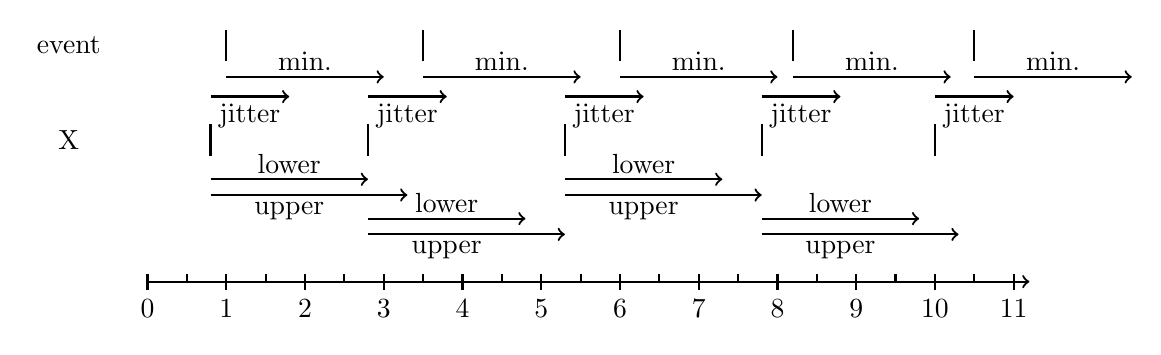
\begin{tikzpicture}[thick]
			% time axis
			\foreach \y in {-2.5}{
				\foreach \x in {0,...,11}
				\draw (\x,\y) -- (\x,\y-0.2) node[anchor=north] {\x};
				\foreach \x in {0.5,1.5,...,10.5}
				\draw (\x,\y) -- (\x,\y-0.1);
				\draw[->] (0,\y-0.1) -- (11.2, \y-0.1);
			}
			% event
			\node at (-1, 0.4) {event};
			\foreach \x in {1, 3.5, 6, 8.2, 10.5}{
				\draw[] (\x,0.2) -- (\x,+0.6);
				%minimum
				\draw[->] (\x, 0) -- (\x+2, 0);
				\node at (\x+1, 0.2) {min.};
			}
			% X
			\node at (-1, -0.8) {X};
			\foreach \x in {0.8, 2.8, 5.3, 7.8, 10}{
				\draw[] (\x,-0.6) -- (\x,-1);
				%jitter
				\draw[->] (\x, -0.25) -- (\x+1, -0.25);
				\node at (\x+0.5, -0.5) {jitter};
			}
			%lower/upper
			\foreach \x in {0.8, 5.3}{
				\node at (\x+1, -1.1){lower};
				\draw[->] (\x, -1.3) -- (\x+2, -1.3);
				\draw[->] (\x, -1.5) -- (\x+2.5, -1.5);
				\node at (\x+1, -1.7){upper};
			}
			\foreach \x in {2.8, 7.8}{
				\node at (\x+1, -1.6){lower};
				\draw[->] (\x, -1.8) -- (\x+2, -1.8);
				\draw[->] (\x, -2) -- (\x+2.5, -2);
				\node at (\x+1, -2.2){upper};
			}

			\end{tikzpicture}
			\caption{Example SporadicConstraint - $lower=2$, $upper=2.5$, $jitter=1$, $minimum=2$}
			\label{fig:SporadicConstraintExample}
		\end{figure}
	
	\subsubsection{PeriodicConstraint}
		The \emph{PeriodicConstraint} takes 4 attribute
		\begin{align*}
			\emph{event} 	& \hspace{.5cm}\text{set of events}\\
			\emph{period} 	& \hspace{.5cm}\mathbb{T}\\
			\emph{jitter}	& \hspace{.5cm}\mathbb{T}\\
			\emph{minimum}	& \hspace{.5cm}\mathbb{T}
		\end{align*}
		and defines a specialized form of the \emph{SporadicConstraint}\\[10pt]
		\begin{math}
			PeriodicConstraint ( event, period, jitter, minimum )\\
			\Leftrightarrow SporadicConstraint(event, period, period, jitter, minimum)
		\end{math}\\[10pt]
		The variable timestamps in the set $X$ are following a strictly periodic pattern, where subsequent elements of this set lay exactly \emph{period} apart. Each element of \emph{event} lays between one element of $X$ and \emph{jitter} after that. Again, there must be bijective mapping between the elements of \emph{event} and $X$.\\
		In figure~\ref{fig:PeriodicConstraintExample}, the \emph{PeriodicConstraint} with the attributes $period=3$, $jitter=1$, $minimum=2.5$ and $event = \{1.2, 4.0, 8, 10.6, ...\}$ is visualized. The timestamps of $X$ lay exactly \emph{period} apart and the $events$ behind that in the previously described way. Also, the minimum time distance between all points of time in \emph{event} is \emph{minimum}.
		\begin{figure}
			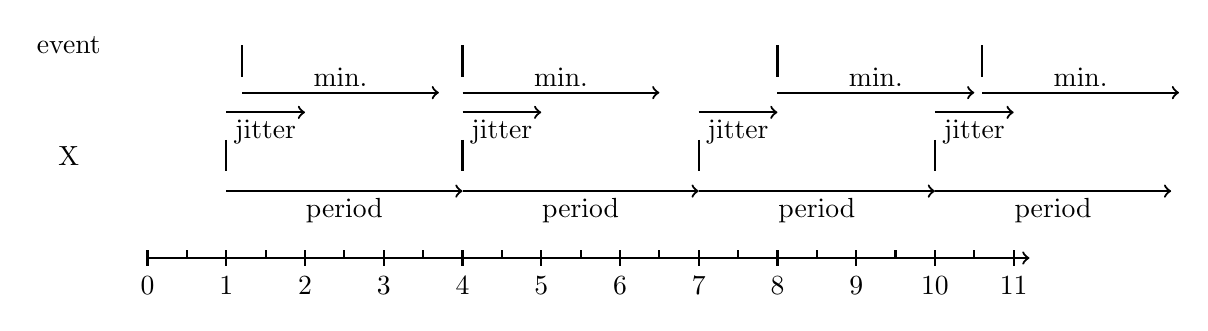
\begin{tikzpicture}[thick]
			% time axis
			\foreach \y in {-2}{
				\foreach \x in {0,...,11}
				\draw (\x,\y) -- (\x,\y-0.2) node[anchor=north] {\x};
				\foreach \x in {0.5,1.5,...,10.5}
				\draw (\x,\y) -- (\x,\y-0.1);
				\draw[->] (0,\y-0.1) -- (11.2, \y-0.1);
			}
			% event
			\node at (-1, 0.6) {event};
			\foreach \x in {1.2, 4.0, 8, 10.6}{
				%timestamp
				\draw[] (\x,0.2) -- (\x,+0.6);
				%minimum
				\draw[->] (\x, 0) -- (\x+2.5, 0);
				\node at (\x+1.25, 0.2) {min.};
			}
			% X
			\node at (-1, -0.8) {X};
			\foreach \x in {1, 4, 7, 10}{
				%timestamp
				\draw[] (\x,-0.6) -- (\x,-1);
				%jitter
				\draw[->] (\x, -0.25) -- (\x+1, -0.25);
				\node at (\x+0.5, -0.5) {jitter};
				%period
				\draw[->] (\x, -1.25) -- (\x+3, -1.25);
				\node at (\x+1.5, -1.5) {period};
			}
			\end{tikzpicture}
			\caption{Example PeriodicConstraint - $period=3$, $jitter=1$, $minimum=2.5$}
			\label{fig:PeriodicConstraintExample}
		\end{figure}
		
		
	\subsubsection{PatternConstraint}
		\label{sec:patterConstraintDefinition}
		The \emph{PatternConstraint} takes 5 attributes
		\begin{align*}
			\emph{event} 	& \hspace{.5cm}\text{set of events}\\
			\emph{period} 	& \hspace{.5cm}\mathbb{T}\\
			\emph{offset}	& \hspace{.5cm} \text{set of }\mathbb{T}\\
			\emph{jitter}	& \hspace{.5cm}\mathbb{T}\\
			\emph{minimum}	& \hspace{.5cm}\mathbb{T}
		\end{align*}
		and is defined as \\[10pt]
		\begin{math}
			PatternConstraint( event, period, \text{\textit{offset}}_1, ..., \text{\textit{offset}}_n, jitter, minimum )\\
			\Leftrightarrow\exists X: PeriodicConstraint(X, period, 0, 0)\\
			\text{\hspace{.5cm}} \land \forall i: DelayContraint(X, event, \text{\textit{offset}}_i,  \text{\textit{offset}}_i+jitter)\\
			\text{\hspace{.5cm}} \land RepeatConstraint(event, minimum, \infty, 1)
		\end{math}\\[10pt]
		This constraint can be understood as a modification of the \emph{PeriodicConstraint}, as it describes periodic behavior, but not from single events, but from groups of $| \text{\textit{offset}}_i|$ subsequent events, that follow specific time distances (specified by $\text{\textit{offset}}$) after the strictly periodic timestamps of $X$.\\
		There is a major weak spot in the definition of this constraint, because the set $X$ can be set to the empty set. In this case, the part of the definition, which uses the \emph{PeriodicConstraint} and the \emph{DelayContraint}, are always satisfied, irrespective of the events in $event$. Therefore, the \emph{PatternConstraint} only ensures the minimal distance between two events, what should not the purpose of this constraint. 
		The obvious countermeasure to this problem would be to restrict $X$ in a way that ensures that it is not empty and the first element of $X$ must lay before the first $event$ occurrence. The textual description of the constraint, which says literally the ''PatternConstraint requires the constrained event occurrences to appear at a predetermined series of offsets from a sequence of reference points'' contradicts this countermeasure, because the \emph{DelayConstraint} allows additional events in the $target$ events with no matching $source$ event. Therefore, any event occurrences additionally to the events following the offset scheme, would be allowed, which conflicts with the citation. Because of this problem, the \emph{PatternConstraint} is redefined as \\[10pt]
		\begin{math}
			PatternConstraint( event, period, \text{\textit{offset}}_1, ..., \text{\textit{offset}}_n, jitter, minimum )\\
			\Leftrightarrow\exists X: PeriodicConstraint(X, period, 0, 0)\\
			\text{\hspace{.5cm}} \land \forall i: \textbf{\emph{Strong}}DelayContraint(X, event, offset_i, offset_i+jitter)\\
			\text{\hspace{.5cm}} \land RepeatConstraint(event, minimum, \infty, 1)
		\end{math}\\[10pt]
		for the scope of this thesis. The use of the \emph{StrongDelayConstraint}, instead of the \emph{DelayConstraint}, ensures that each event occurrence is following the time distances defined by the offsets. This notion of the \emph{PatternConstraint} is also carried by the described relations between the TADL2 timing constraints and the AUTOSAR Timing Extensions, which were done as part of the development of TADL2\cite{TIMMO2USE}. These descriptions equate the \emph{PatternConstraint} and AUTOSARs \emph{ConcretePatternEventTriggering}, which is clearly defined in the way of this redefinition.\\
		Figure~\ref{fig:PatternConstraintExample} shows an application of the \emph{PeriodicConstraint} with the attributes $period=5$, $\text{\textit{offset}}=\{1, 2, 2.5\}$, $jitter=0.5$, $minimum=0.5$ and\\
		$event = \{1.2, 2.2, 2.8, 6, 7, 8, 11.5, 12, 12.5, ...\}$. Like in the previous describes constraint, the exact position of all points in time of $X$ may change due to later timestamps of $event$.
		\begin{figure}
			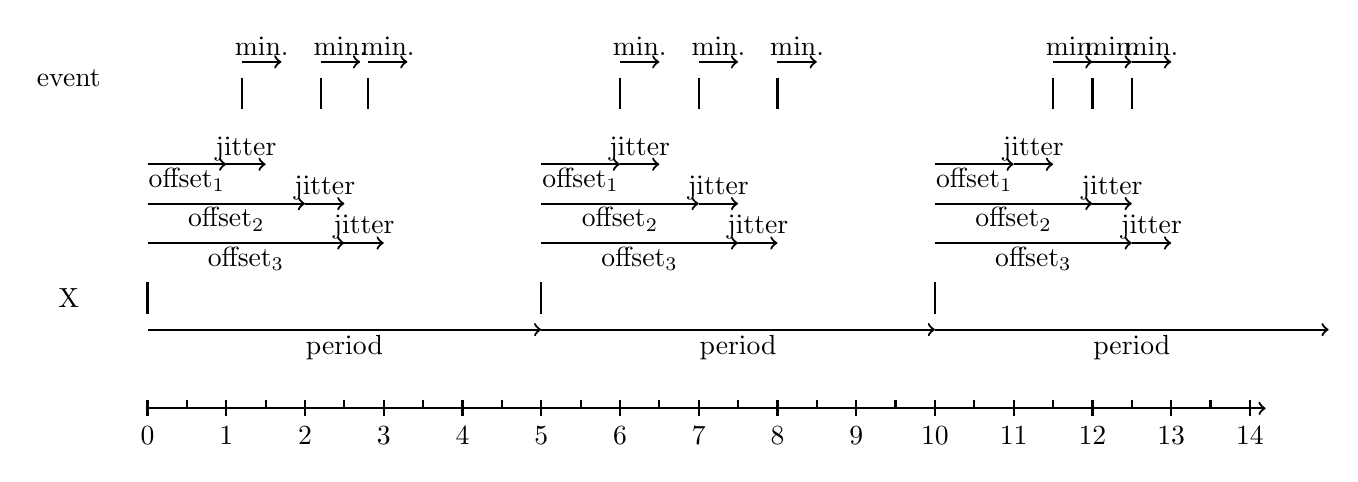
\begin{tikzpicture}[thick]
			% time axis
			\foreach \y in {-3.5}{
				\foreach \x in {0,...,14}
				\draw (\x,\y) -- (\x,\y-0.2) node[anchor=north] {\x};
				\foreach \x in {0.5,1.5,...,13.5}
				\draw (\x,\y) -- (\x,\y-0.1);
				\draw[->] (0,\y-0.1) -- (14.2, \y-0.1);
			}
			% event
			\node at (-1, 0.6) {event};
			\foreach \x in {1.2, 2.2, 2.8, 6, 7, 8, 11.5, 12, 12.5}{
				%timestamp
				\draw[] (\x,0.2) -- (\x,+0.6);
				%minimum
				\draw[->] (\x, 0.8) -- (\x+.5, 0.8);
				\node at (\x+0.25, 1) {min.};
			}
			% X
			\node at (-1, -2.2) {X};
			\foreach \x in {0,5, 10}{
				%timestamp
				\draw[] (\x,-2) -- (\x,-2.4);
				%offset 1
				\draw[->] (\x, -0.5) -- (\x+1, -0.5);
				\node at (\x+0.5, -0.7) {offset$_1$};
				\draw[->] (\x+1, -0.5) -- (\x+1.5, -0.5);
				\node at (\x+1.25, -0.3) {jitter};
				%offset 2
				\draw[->] (\x, -1) -- (\x+2, -1);
				\node at (\x+1, -1.2) {offset$_2$};
				\draw[->] (\x+2, -1) -- (\x+2.5, -1);
				\node at (\x+2.25, -0.8) {jitter};
				%offset 3
				\draw[->] (\x, -1.5) -- (\x+2.5, -1.5);
				\node at (\x+1.25, -1.7) {offset$_3$};
				\draw[->] (\x+2.5, -1.5) -- (\x+3, -1.5);
				\node at (\x+2.75, -1.3) {jitter};
				%period
				\draw[->] (\x, -2.6) -- (\x+5, -2.6);
				\node at (\x+2.5, -2.83) {period};
			}
			\end{tikzpicture}
			\caption{Example PatternConstraint - $period=5$, $offset=\{1, 2, 2.5\}$, $jitter=0.5$, $minimum=0.5$}
			\label{fig:PatternConstraintExample}
		\end{figure}
		
	\subsubsection{ArbitraryConstraint}
		The \emph{ArbitraryConstraint} takes 3 attributes
		\begin{align*}
			\emph{event} 	& \hspace{.5cm}\text{set of events}\\
			\emph{minimum}	& \hspace{.5cm}\text{set of }\mathbb{T}\\
			\emph{maximum}	& \hspace{.5cm}\text{set of }\mathbb{T}
		\end{align*}
		where $|minimum|=|maximum|$. It is defined as \\[10pt]
		\begin{math}\\
			ArbitraryConstraint ( event, minimum_1, ..., minimum_n, maximum_1, ..., maximum_n)\\
			\Leftrightarrow\forall i: RepeatConstraint(event, minimum_i, maximum_i, i)
		\end{math}\\[10pt]
		The Idea behind the \emph{ArbitraryConstraint} is to describe the time distance between each event and several following events. The first entry of \emph{minimum} and \emph{maximum} define the distance between every event and it direct successor. The second entries, where the \emph{span} attribute of the  \emph{RepeatConstraint} is 2, defines the distance between one event and its next but one successor and so on.\\
		Figure~\ref{fig:ArbitraryConstraintExample} shows an example of the \emph{ArbitraryConstraint} with the attributes $minimum=\{1,2,3\}$, $maximum=\{5,6,7\}$ and $event=\{1, 2, 3, 5, 8, 10, ...\}$. The time distances between subsequent events with 0, 1, 2 and more skipped events are shown in table~\ref{tab:ArbitraryConstraintExampleTable}, the relevant distances are written in \textbf{bold} font. Apparently, the time distances are matching the ranges, given by the $minimum$- and $maximum$ attribute.\\
		\begin{table}
			\begin{tabular}{|c|c|c|c|c|c|c|}
				\hline
				& 1 & 2 & 3 & 5 & 8 & 10 \\
				\hline
				1 & 0 & \textbf{1} & \textbf{2} & \textbf{4} & 7 & 9 \\
				\hline
				2 &  & 0 & \textbf{1} & \textbf{3} & \textbf{6} & 8 \\
				\hline
				3 &  &  & 0 & \textbf{2} & \textbf{5} & \textbf{7} \\
				\hline
				5 &  &  &  & 0 & \textbf{3} & \textbf{5} \\
				\hline
				8 &  &  &  &  & 0 & \textbf{2} \\
				\hline
				10 &  &  &  &  &  & 0 \\
				\hline
			\end{tabular}
			\centering
			\caption{Time distances as seen in figure~\ref{fig:ArbitraryConstraintExample}}
			\label{tab:ArbitraryConstraintExampleTable}
		\end{table}

		\begin{figure}
			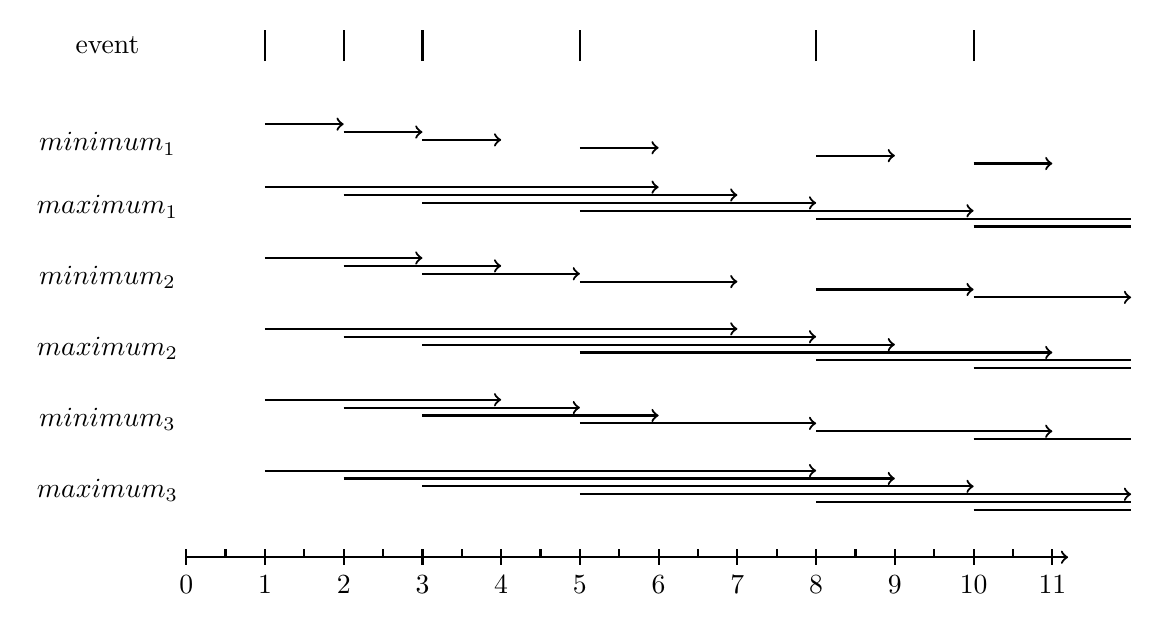
\begin{tikzpicture}[thick]
			% time axis
			\foreach \y in {-6}{
				\foreach \x in {0,...,11}
				\draw (\x,\y) -- (\x,\y-0.2) node[anchor=north] {\x};
				\foreach \x in {0.5,1.5,...,10.5}
				\draw (\x,\y) -- (\x,\y-0.1);
				\draw[->] (0,\y-0.1) -- (11.2, \y-0.1);
			}
			% event
			\node at (-1, 0.4) {event};
			\node at (-1, -0.85) {$minimum_1$};
			\node at (-1, -1.65) {$maximum_1$};
			
			\node at (-1, -2.55) {$minimum_2$};
			\node at (-1, -3.45) {$maximum_2$};
			
			
			\node at (-1, -4.35) {$minimum_3$};
			\node at (-1, -5.25) {$maximum_3$};
			\foreach \x in {1,2,3,5,8,10}{
				%timestamp
				\draw[] (\x,0.2) -- (\x,+0.6);
			}
			% minimum 1
			\draw[->] (1, -0.6) -- (2, -0.6);
			\draw[->] (2, -0.7) -- (3, -0.7);
			\draw[->] (3, -0.8) -- (4, -0.8);
			\draw[->] (5, -0.9) -- (6, -0.9);
			\draw[->] (8, -1.0) -- (9, -1.0);
			\draw[->] (10, -1.1) -- (11, -1.1);
			% maximum 1
			\draw[->] (1, -1.4) -- (6, -1.4);
			\draw[->] (2, -1.5) -- (7, -1.5);
			\draw[->] (3, -1.6) -- (8, -1.6);
			\draw[->] (5, -1.7) -- (10, -1.7);
			\draw[-] (8, -1.8) -- (12, -1.8);
			\draw[-] (10, -1.9) -- (12, -1.9);
			
			% minimum 2
			\draw[->] (1, -2.3) -- (3, -2.3);
			\draw[->] (2, -2.4) -- (4, -2.4);
			\draw[->] (3, -2.5) -- (5, -2.5);
			\draw[->] (5, -2.6) -- (7, -2.6);
			\draw[->] (8, -2.7) -- (10, -2.7);
			\draw[->] (10, -2.8) -- (12, -2.8);
			
			% maximum 2
			\draw[->] (1, -3.2) -- (7, -3.2);
			\draw[->] (2, -3.3) -- (8, -3.3);
			\draw[->] (3, -3.4) -- (9, -3.4);
			\draw[->] (5, -3.5) -- (11, -3.5);
			\draw[-] (8, -3.6) -- (12, -3.6);
			\draw[-] (10, -3.7) -- (12, -3.7);
			
			% minimum 3
			\draw[->] (1, -4.1) -- (4, -4.1);
			\draw[->] (2, -4.2) -- (5, -4.2);
			\draw[->] (3, -4.3) -- (6, -4.3);
			\draw[->] (5, -4.4) -- (8, -4.4);
			\draw[->] (8, -4.5) -- (11, -4.5);
			\draw[-] (10, -4.6) -- (12, -4.6);
			
			% maximum 3
			\draw[->] (1, -5.0) -- (8, -5.0);
			\draw[->] (2, -5.1) -- (9, -5.1);
			\draw[->] (3, -5.2) -- (10, -5.2);
			\draw[->] (5, -5.3) -- (12, -5.3);
			\draw[-] (8, -5.4) -- (12, -5.4);
			\draw[-] (10, -5.5) -- (12, -5.5);
			
			
			\end{tikzpicture}
			\caption{Example ArbitraryConstraint - $minimum=\{1,2,3\}$ and $minimum=\{4,5,6\}$}
			\label{fig:ArbitraryConstraintExample}
		\end{figure}
		
	\subsubsection{BurstConstraint}
		The \emph{BurstConstraint} takes 4 attributes
		\begin{align*}
			\emph{event} 			& \hspace{.5cm}\text{set of events}\\
			\emph{length}			& \hspace{.5cm} \mathbb{T}\\
			\emph{maxOccurrences}	& \hspace{.5cm} integer\\
			\emph{minimum}			& \hspace{.5cm} \mathbb{T}
		\end{align*}
		and is defined as \\[10pt]
		\begin{math}
			BurstConstraint ( event, length, maxOccurrences, minimum )\\
			\Leftrightarrow RepeatConstraint(event, length, \infty, maxOccurrences)\\
			\text{\hspace{.5cm}}\land RepeatConstraint(event, minimum, \infty, 1)
		\end{math}\\[10pt]
		 The idea of this constraint is to describe the maximum number of events that may occur in a time interval of the given $length$. Additionally all subsequent event must be at least \emph{minimum} apart. Therefore, the intuition is different to the AUTOSAR \emph{BurstPatternEventTriggering}, where clusters of events are described. A complete comparison of these constraints will be done in section~\ref{comparisonConstraints}.\\
		 In figure~\ref{fig:BurstConstraintExample}, an application of the \emph{BurstConstraint} with the attributes $length=5$, $maxOccurrences=3$, $minimum=0.8$ and $event = \{1,2,3,7,8,9\}$ is visualized. In every interval of the length 5, there are three or less events, also all subsequent events lay at least $0.8$ apart. Therefore, the constraint is fulfilled.
 		\begin{figure}
		 	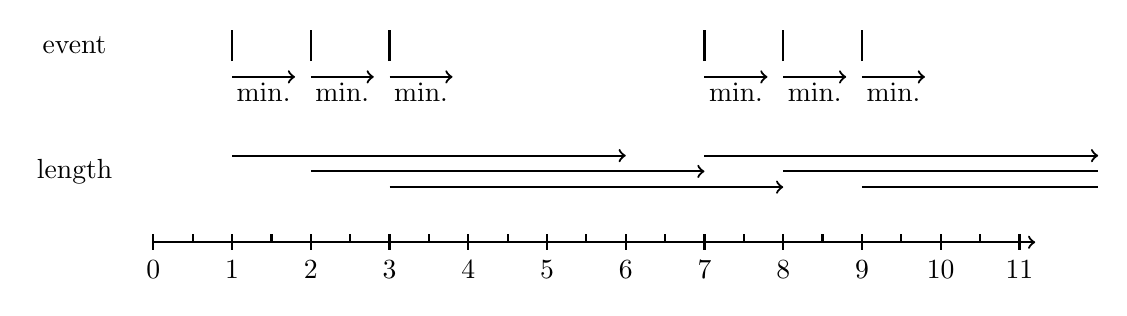
\begin{tikzpicture}[thick]
			 	% time axis
			 	\foreach \y in {-2}{
			 		\foreach \x in {0,...,11}
			 		\draw (\x,\y) -- (\x,\y-0.2) node[anchor=north] {\x};
			 		\foreach \x in {0.5,1.5,...,10.5}
			 		\draw (\x,\y) -- (\x,\y-0.1);
			 		\draw[->] (0,\y-0.1) -- (11.2, \y-0.1);
			 	}
			 	% event
			 	\node at (-1, 0.4) {event};
			 	\foreach \x in {1, 2, 3, 7, 8, 9}{
			 		%timestamp
			 		\draw[] (\x,0.2) -- (\x,+0.6);
			 		%minimum
			 		\draw[->] (\x, 0) -- (\x+0.8, 0);
			 		\node at (\x+0.4, -0.2) {min.};
			 	}
		 		% length
		 		\node at (-1, -1.2) {length};
		 		\draw[->] (1, -1) -- (6, -1);
	 			\draw[->] (2, -1.2) -- (7, -1.2);
 				\draw[->] (3, -1.4) -- (8, -1.4);
 				\draw[->] (7, -1) -- (12, -1);
 				\draw[-] (8, -1.2) -- (12, -1.2);
 				\draw[-] (9, -1.4) -- (12, -1.4);
		 	\end{tikzpicture}
		 	\caption{Example BurstConstraint - $length=5$, $maxOccurences=3$ $minimum=0.8$}
		 	\label{fig:BurstConstraintExample}
		 \end{figure}
	
	\subsubsection{ReactionConstraint}
		The \emph{ReactionConstraint} takes 3 attributes
		\begin{align*}
			\emph{scope} 	& \hspace{.5cm} EventChain\\
			\emph{minimum}	& \hspace{.5cm} \mathbb{T}\\
			\emph{maximum}	& \hspace{.5cm} \mathbb{T}
		\end{align*}
		and is defined as \\[10pt]
		\begin{math}
			ReactionConstraint ( scope, minimum, maximum )\\
			\Leftrightarrow\forall x\in scope.stimulus: \exists y\in scope.response:\\
			\text{\hspace{.5cm}}x.color=y.color\\
			\text{\hspace{.5cm}}\land (\forall y'\in scope.response: y'.color=y.color\Rightarrow y\leq y')\\
			\text{\hspace{.5cm}}\land minimum \leq y-x \leq maximum
		\end{math}\\[10pt]
		The definition says that after every event $x$ of $scope.stimulus$, there is an event $y$ in $scope.response$ with the same color. The time distance between these events must be at least $minimum$ and at most $maximum$. Additional events with the same color as $y$ in $scope.response$ are allowed, if they lay behind $y$.  The definition implies that additional events with other colors are allowed in $scope.response$, but not in $scope.stimulus$.\\
		A visualized example with the attributes $minimum=1$, $maximum=3$,\\
		$scope.stimulus=\{(1, red), (5, green), (5.5, purple), (8, orange)\}$ and $scope.response=\{(0.8, blue), (2.1, red), (4.5, blue), (6.6, purple),
		(6.7, purple), (9.5, purple), (7.5, green), \\
		(10, orange)\}$ can be seen in figure~\ref{fig:ReactionConstraint}. The red $stimulus$ event is followed by the red $response$-event at 2.1, the green $stimulus$ event at 5 by the $response$ event at 7.5 and so on. The blue $response$ events at 1 and 4.5 are additional events without an associated stimulus event. The purple events at 6.7 and 9.5 are the second and third event of this color in $scope.response$ and therefore, their time distance to the $stimulus$ event with the same color is irrelevant.
 		\begin{figure}
			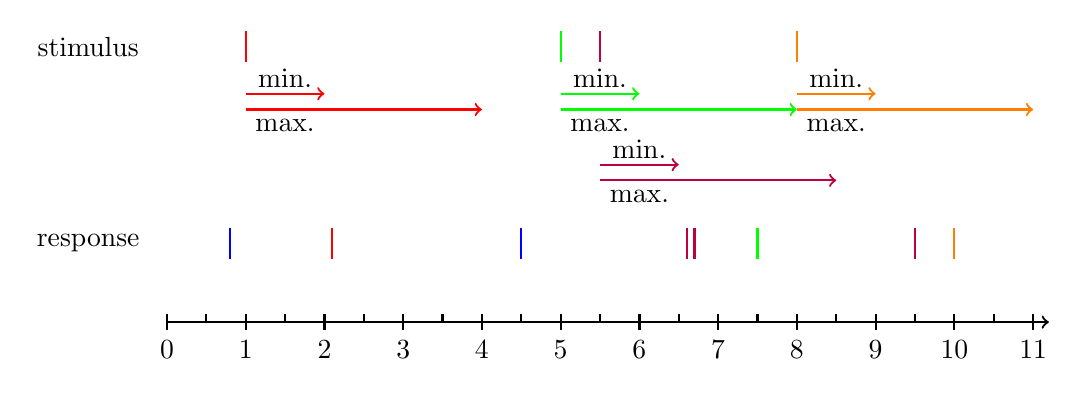
\begin{tikzpicture}[thick]
				% time axis
				\foreach \y in {-3}{
					\foreach \x in {0,...,11}
					\draw (\x,\y) -- (\x,\y-0.2) node[anchor=north] {\x};
					\foreach \x in {0.5,1.5,...,10.5}
					\draw (\x,\y) -- (\x,\y-0.1);
					\draw[->] (0,\y-0.1) -- (11.2, \y-0.1);
				}
				% stimulus
				\node at (-1, 0.4) {stimulus};
				\draw[red, thick]    (1  ,0.2) -- (1,+0.6);
				\draw[green, thick]  (5  ,0.2) -- (5,+0.6);
				\draw[purple, thick] (5.5,0.2) -- (5.5,+0.6);
				\draw[orange, thick] (8  ,0.2) -- (8,+0.6);
				
				% minimum
				\draw[->, red] (1, -0.2) -- (2, -0.2);
				\node at (1.5, 0) {min.};
				\draw[->, green] (5, -0.2) -- (6, -0.2);
				\node at (5.5, 0) {min.};
				\draw[->, purple] (5.5, -1.1) -- (6.5, -1.1);
				\node at (6, -0.9) {min.};
				\draw[->, orange] (8, -0.2) -- (9, -0.2);
				\node at (8.5, 0) {min.};
				%maximum
				\draw[->, red] (1, -0.4) -- (4, -0.4);
				\node at (1.5, -0.6) {max.};
				\draw[->, green] (5, -0.4) -- (8, -0.4);
				\node at (5.5, -0.6) {max.};
				\draw[->, purple] (5.5, -1.3) -- (8.5, -1.3);
				\node at (6, -1.5) {max.};
				\draw[->, orange] (8, -0.4) -- (11, -0.4);
				\node at (8.5, -0.6) {max.};
				%response
				\node at (-1, -2.1) {response};
				\draw[blue, thick]    (.8  ,-1.9) -- (.8,-2.3);
				\draw[blue, thick]    (4.5  ,-1.9) -- (4.5,-2.3);
				\draw[red, thick]    (2.1  ,-1.9) -- (2.1,-2.3);
				\draw[green, thick]  (7.5  ,-1.9) -- (7.5,-2.3);
				\draw[purple, thick] (6.6,-1.9) -- (6.6,-2.3);
				\draw[purple, thick] (6.7,-1.9) -- (6.7,-2.3);
				\draw[purple, thick] (9.5,-1.9) -- (9.5,-2.3);
				\draw[orange, thick] (10  ,-1.9) -- (10,-2.3);
			\end{tikzpicture}
			\caption{Example ReactionConstraint - $minimum=1$, $maximum=3$}
			\label{fig:ReactionConstraint}
		\end{figure}
		
	
	\subsubsection{AgeConstraint}
		The \emph{AgeConstraint} takes 3 attributes
		\begin{align*}
			\emph{scope} 	& \hspace{.5cm} EventChain\\
			\emph{minimum}	& \hspace{.5cm} \mathbb{T}\\
			\emph{maximum}	& \hspace{.5cm} \mathbb{T}
		\end{align*}
		and is defined as \\[10pt]
		\begin{math}
			AgeConstraint ( scope, minimum, maximum )\\
			\Leftrightarrow\forall y\in scope.response: \exists x\in scope.stimulus:\\
			\text{\hspace{.5cm}}x.color=y.color\\
			\text{\hspace{.5cm}}\land (\forall x'\in scope.stimulus: x'.color=x.color\Rightarrow x'\leq x)\\
			\text{\hspace{.5cm}}\land minimum \leq y-x \leq maximum
		\end{math}\\[10pt]
		The \emph{AgeConstraint} is a turned around counterpart to the \emph{ReactionConstraint}. For every event of $scope.response$, there must be an event with the same color in $scope.stimulus$, that is between $minimum$ and $maximum$ older than the $response$ event. Additional events are only allowed in $scope.stimulus$, and only before the event that matches with a $response$ event, which is implied by the correctness of the event chain.\\
		Figure~ \ref{fig:AgeConstraint} shows an application of the \emph{AgeConstraint} with the attributes $minimum=1$, $maximum=3$, $scope.stimulus=\{(0.8, blue), (1, red), (2, green), (4.5, green),\\
		(5, green), (5.5, purple), (8, orange)\}$ and $scope.response=\{(3.5, red), (7.5, green),\\
		 (6.6, purple), (10, orange)\}$. The blue timestamps are additional events without matching events in $scope.response$.
 		\begin{figure}
			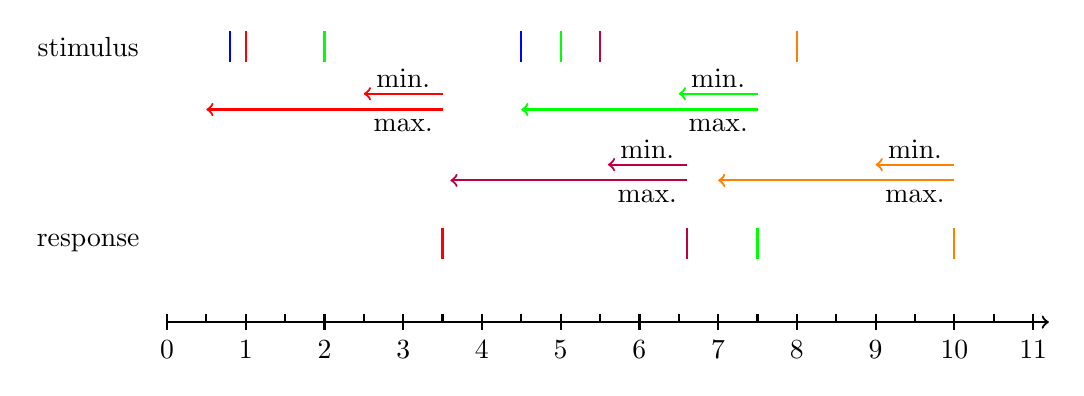
\begin{tikzpicture}[thick]
				% time axis
				\foreach \y in {-3}{
					\foreach \x in {0,...,11}
					\draw (\x,\y) -- (\x,\y-0.2) node[anchor=north] {\x};
					\foreach \x in {0.5,1.5,...,10.5}
					\draw (\x,\y) -- (\x,\y-0.1);
					\draw[->] (0,\y-0.1) -- (11.2, \y-0.1);
				}
				% stimulus
				\node at (-1, 0.4) {stimulus};
				\draw[red, thick]    (1  ,0.2) -- (1,+0.6);
				\draw[green, thick]  (2  ,0.2) -- (2,+0.6);
				\draw[green, thick]  (5  ,0.2) -- (5,+0.6);
				\draw[purple, thick] (5.5,0.2) -- (5.5,+0.6);
				\draw[orange, thick] (8  ,0.2) -- (8,+0.6);
				\draw[blue, thick] (0.8, 0.2) -- (0.8,0.6);
				\draw[blue, thick] (4.5, 0.2) -- (4.5,0.6);
				
				% minimum
				\draw[->, red] (3.5, -0.2) -- (2.5, -0.2);
				\node at (3, 0) {min.};
				\draw[->, green] (7.5, -0.2) -- (6.5, -0.2);
				\node at (7, 0) {min.};
				\draw[->, purple] (6.6, -1.1) -- (5.6, -1.1);
				\node at (6.1, -0.9) {min.};
				\draw[->, orange] (10, -1.1) -- (9, -1.1);
				\node at (9.5, -0.9) {min.};
				%maximum
				\draw[->, red] (3.5, -0.4) -- (0.5, -0.4);
				\node at (3, -0.6) {max.};
				\draw[->, green] (7.5, -0.4) -- (4.5, -0.4);
				\node at (7, -0.6) {max.};
				\draw[->, purple] (6.6, -1.3) -- (3.6, -1.3);
				\node at (6.1, -1.5) {max.};
				\draw[->, orange] (10, -1.3) -- (7, -1.3);
				\node at (9.5, -1.5) {max.};
				%response
				\node at (-1, -2.1) {response};
				\draw[red, thick]    (3.5  ,-1.9) -- (3.5,-2.3);
				\draw[green, thick]  (7.5  ,-1.9) -- (7.5,-2.3);
				\draw[purple, thick] (6.6,-1.9) -- (6.6,-2.3);
				%\draw[purple, thick] (6.7,-1.9) -- (6.7,-2.3);
				%\draw[purple, thick] (9.5,-1.9) -- (9.5,-2.3);
				\draw[orange, thick] (10  ,-1.9) -- (10,-2.3);
			\end{tikzpicture}
			\caption{Example AgeConstraint - $minimum=1$, $maximum=3$}
			\label{fig:AgeConstraint}
		\end{figure}
		
	\subsubsection{OutputSynchronizationConstraint}
		The \emph{OutputSynchronizationConstraint} takes 2 attributes
		\begin{align*}
			\emph{scope} 	& \hspace{.5cm} \text{Set of }EventChain\\
			\emph{tolerance}	& \hspace{.5cm} \mathbb{T}
		\end{align*}
		where all elements of \emph{scope} have the same $stimulus$ event set. It is defined as \\[10pt]
		\begin{math}
			OutputSynchronizationConstraint ( scope_1, ..., scope_n, tolerance )\\
			\Leftrightarrow\forall x\in scope_1.stimulus: \exists t: \forall i: \exists y\in scope_i.response:\\
			\text{\hspace{.5cm}} x.color = y.color\\
			\text{\hspace{.5cm}}\land (\forall y'\in scope_i.response: y'.color=y.color \Rightarrow y\leq y')\\
			\text{\hspace{.5cm}}\land 0\leq y-t\leq tolerance
		\end{math}\\[10pt]
		The definition says, that after each event $x$ in $scope_1.stimulus$, there must be a interval with the length of $tolerance$, in which every $scope_i.response$ must have an event $y$ with the same color as $x$. Additional response events with this color are only allowed after $y$.
		Figure~\ref{fig:OutputSynchronizationConstraint} shows an example of the \emph{OutputSynchronizationConstraint} with the attributes $tolerance = 1$,\\
		 $scope[1].stimulus=scope[2].stimulus=scope[3].stimulus=\{(1, red), (4, green), (5, purple)\}$,\\
		$scope[1].response=\{(2, red), (6, purple), (6.2, purple), (8.2, green)\}$,\\
		$scope[2].response=\{(2.6, red), (6.2, purple), (8, green), (10.5, green)\}$,\\
		$scope[3].response=\{(2.3, red), (6.5, purple), (8.5, green)\}$.\\
		
 		\begin{figure}
			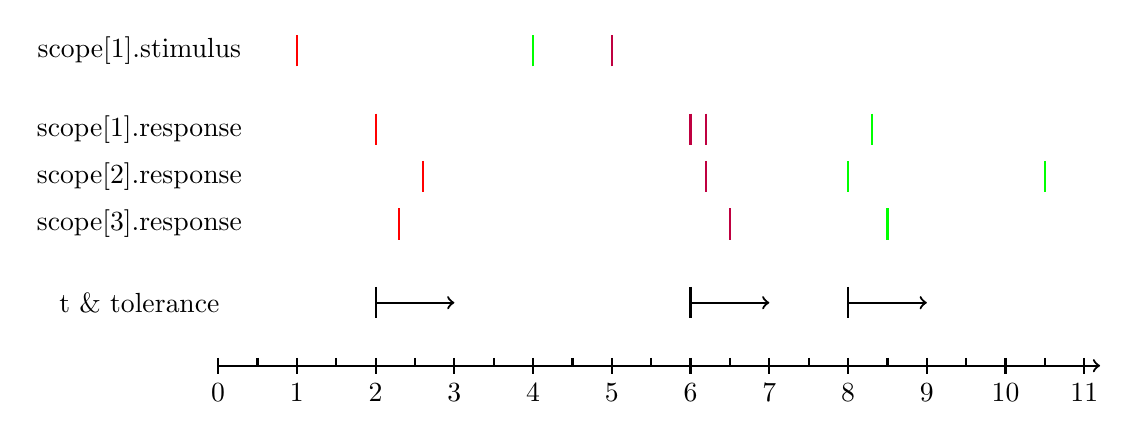
\begin{tikzpicture}[thick]
				% time axis
				\foreach \y in {-3.5}{
					\foreach \x in {0,...,11}
					\draw (\x,\y) -- (\x,\y-0.2) node[anchor=north] {\x};
					\foreach \x in {0.5,1.5,...,10.5}
					\draw (\x,\y) -- (\x,\y-0.1);
					\draw[->] (0,\y-0.1) -- (11.2, \y-0.1);
				}
				% stimulus
				\node at (-1, 0.4) {scope\textcolor{black}{[1]}.stimulus};
				\draw[red, thick]    (1  ,0.2) -- (1,+0.6);
				\draw[green, thick]  (4  ,0.2) -- (4,+0.6);
				\draw[purple, thick] (5,0.2) -- (5,+0.6);
				
				\node at(-1, -0.6) {scope[1].response};
				\draw[red, thick]    (2, -0.4) -- (2, -0.8);
				\draw[green, thick]  (8.3, -0.4) -- (8.3, -0.8);
				\draw[purple, thick] (6, -0.4) -- (6, -0.8);
				\draw[purple, thick] (6.2, -0.4) -- (6.2, -0.8);
				
				\node at(-1, -1.2) {scope[2].response};
				\draw[red, thick]    (2.6, -1) -- (2.6, -1.4);
				\draw[green, thick]    (8, -1) -- (8, -1.4);
				\draw[green, thick]    (10.5, -1) -- (10.5, -1.4);
				\draw[purple, thick]    (6.2, -1) -- (6.2, -1.4);
				
				\node at(-1, -1.8) {scope[3].response};
				\draw[red, thick]    (2.3, -1.6) -- (2.3, -2);
				\draw[green, thick]  (8.5, -1.6) -- (8.5, -2);
				\draw[purple, thick] (6.5, -1.6) -- (6.5, -2);
				
				\node at (-1, -2.8) {t \& tolerance};
				\foreach \i in {2, 6, 8} {
					\draw[thick] (\i, -2.6) -- (\i, -3);
					\draw[->] (\i, -2.8) -- (\i+1, -2.8);
				}

			\end{tikzpicture}
			\caption{Example OutputSynchronizationConstraint - $tolerance=1$}
			\label{fig:OutputSynchronizationConstraint}
		\end{figure}
		
	\subsubsection{InputSynchronizationConstraint}
	The \emph{InputSynchronizationConstraint} takes 2 attributes
	\begin{align*}
		\emph{scope} 	& \hspace{.5cm} \text{Set of }EventChain\\
		\emph{tolerance}& \hspace{.5cm} \mathbb{T}
	\end{align*}
	where all elements of \emph{scope} have the same $response$ event set. It is defined as \\[10pt]
	\begin{math}\\
		InputSynchronizationConstraint ( scope_1, ..., scope_n, tolerance )\\
		\Leftrightarrow\forall y\in scope_1.response: \exists t: \forall i: \exists x\in scope_i.stimulus:\\
		\text{\hspace{.5cm}} x.color = y.color\\
		\text{\hspace{.5cm}}\land (\forall x'\in scope_i.stimulus: x'.color=x.color \Rightarrow x\leq x')\\
		\text{\hspace{.5cm}}\land 0\leq x-t\leq tolerance
	\end{math}\\[10pt]
	The \emph{InputSynchronizationConstraint} is a counterpart of the \emph{OutputSynchronizationConstraint}, as the \emph{stimulus} events must be synchronized, not the \emph{response} events.\\
	Figure~\ref{fig:InputSynchronizationConstraint} contains an example of the \emph{InputSynchronizationConstraint} with the attributes $tolerance=1$\\
	$scope[1].stimulus=\{(1, red), (1.5, green), (4.6, green), (8, purple)\}$\\
	$scope[2].stimulus=\{(1.2, red), (4, green), (8.3, purple), (8.5, purple)\}$\\
	$scope[3].stimulus=\{(1.5, red), (4, green), (8.9, purple)\}$\\
	$scope[1].response=scope[2].response=scope[3].response=\{(2.5, red), (6, green), (10, purple)\}$\\
	\begin{figure}
		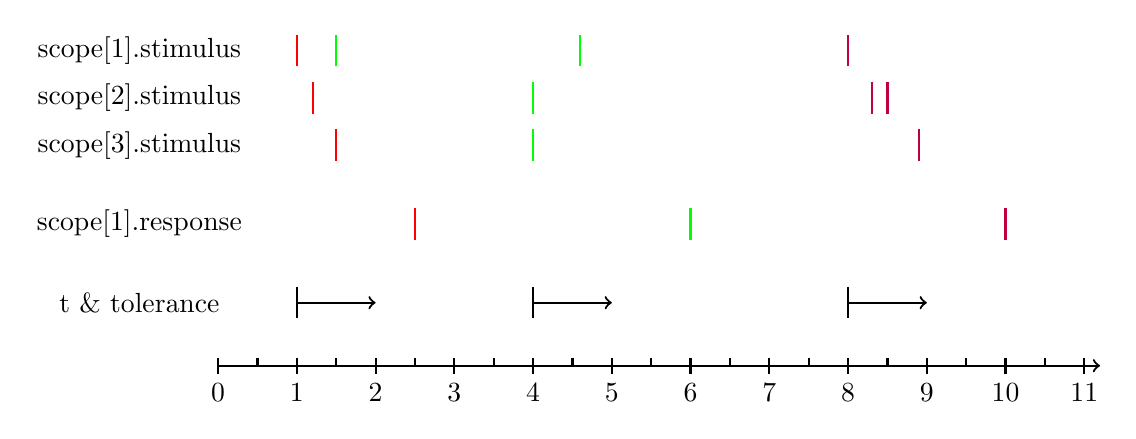
\begin{tikzpicture}[thick]
			% time axis
			\foreach \y in {-3.5}{
				\foreach \x in {0,...,11}
				\draw (\x,\y) -- (\x,\y-0.2) node[anchor=north] {\x};
				\foreach \x in {0.5,1.5,...,10.5}
				\draw (\x,\y) -- (\x,\y-0.1);
				\draw[->] (0,\y-0.1) -- (11.2, \y-0.1);
			}
			% stimulus
			\node at (-1, 0.4) {scope[1].stimulus};
			\draw[red, thick]    (1  ,0.2) -- (1,+0.6);
			\draw[green, thick]  (1.5  ,0.2) -- (1.5,+0.6);
			\draw[green, thick]  (4.6  ,0.2) -- (4.6,+0.6);
			\draw[purple, thick] (8,0.2) -- (8,+0.6);
			
			\node at (-1, -0.2) {scope[2].stimulus};
			\draw[red, thick]    (1.2,0) -- (1.2, -0.4);
			\draw[green, thick]  (4  ,0) -- (4,-0.4);
			\draw[purple, thick] (8.3,  0) -- (8.3,-0.4);
			\draw[purple, thick] (8.5,  0) -- (8.5,-0.4);
			
			\node at (-1, -0.8) {scope[3].stimulus};
			\draw[red, thick]    (1.5,-0.6) -- (1.5, -1);
			\draw[green, thick]  (4,  -0.6) -- (4,-1);
			\draw[purple, thick] (8.9,-0.6) -- (8.9,-1);
			
			\node at(-1, -1.8) {scope[1].response};
			\draw[red, thick]    (2.5, -1.6) -- (2.5, -2);
			\draw[green, thick]  (6, -1.6) -- (6, -2);
			\draw[purple, thick] (10, -1.6) -- (10, -2);
			
			\node at (-1, -2.8) {t \& tolerance};
			\foreach \i in {1, 4, 8} {
				\draw[thick] (\i, -2.6) -- (\i, -3);
				\draw[->] (\i, -2.8) -- (\i+1, -2.8);
			}
			
		\end{tikzpicture}
		\caption{Example InputSynchronizationConstraint - $tolerance=1$}
		\label{fig:InputSynchronizationConstraint}
	\end{figure}
			
\subsection{Comparison TADL2 - AUTOSAR Timing Extension}
\label{comparisonConstraints}
	As said before, the \emph{TADL2 Timing Constraints} and the \emph{AUTOSAR Timing Extensions} are compatible in parts and many of the \emph{AUTOSAR Timing Extension} can be expressed as equivalent combinations of the \emph{TADL2 Timing Constraints}. In \cite{TIMMO2USE}, the relation between these constraints is shown, but this comparison is based on an outdated version of the AUTOSAR Timing Extensions and some of the constraints have been updated, therefore each of the \emph{AUTOSAR Timing Extensions} will be listed in this chapter and it will be explained, if and how they can be expressed using \emph{TADL2 Timing Constraints}.\\
	The types used in the AUTOSAR Timing Extension are similar to the ones in TADL2. TADL2 \emph{Events} are called \emph{TimingDescriptionEvent} in AUTOSAR, the same goes for \emph{EventChains}, which are called \emph{TimingDescriptionEventChains}. A larger difference can be seen in the definition of time. While TADL2 defines time as real numbers, the time definition used in the AUTOSAR Timing Extension can also be multidimensional, for example when the real time and the angle of the crankshaft is regarded. For simplification, all timestamps are considered as real numbers in the following, but an extension to multidimensional time stamps is possible, as AUTOSAR requires a strict order between all time stamps. Some of the AUTOSAR Timing Extensions are defined on \emph{Executable Entities}, describe things, that can be executed, for example a function. In the analysis of their timing, only striking points in times of these entities are relevant, for example the start or end points, therefore \emph{Executable Entities} can be transformed into events if needed.
	
	It should be noted, that the set of TADL2 timing constraints are not equal to the AUTOSAR Timing Extension and that there are constraints, that cannot be expressed using the corresponding counterpart.

	\subsubsection{PeriodicEventTriggering}
		The \emph{PeriodicEventTriggering} defined in AUTOSAR with the attributes\\ $(\textcolor{black}{event}, period, jitter, minimumInterArrivalTime)$ is equivalent to the \emph{TADL2} \emph{PeriodicConstraint} with the same attributes.
		
	\subsubsection{SporadicEventTriggering}
		AUTOSARs \emph{SporadicEventTriggering} with the attributes\\
		 $(\textcolor{black}{event}, jitter, maximumInterArrivalTime,  minimumInterArrivalTime, period)$ is equivalent to the \emph{TADL2} \emph{SporadicConstraint}, but the names of the attributes are different:\\
		\begin{math}
			lower\widehat{=}period\\
			upper\widehat{=}maximumInterArrivalTime\\
			jitter\widehat{=}jitter\\
			minimum\widehat{=}minimumInterArrivalTime
		\end{math}
	
	\subsubsection{ConcretePatternEventTriggering}
		The idea behind the \emph{ConcretePatternEventTriggering} from \textit{AUTOSAR} is the same as behind \textit{TADL2s} \emph{PatternConstraint}, but some details are different. Both define a periodic behavior and offsets, that describe time distances between the periods and the actual events. The main difference is the \emph{jitter} attribute. In AUTOSARs \emph{ConcretePatternEventTriggering}, the \emph{patternJitter} attribute defines the allowed deviation of the start points from the periodic repetitions, but in TADL2 the $jitter$ value describes the deviation between the offsets and the actual event.\\
		The \emph{ConcretePatternEventTriggering} from AUTOSAR additionally defines an \emph{patternLength} attribute, which describes the length of the intervals, in which the clusters of events will occur. It is constrained by\\[10pt]
		\begin{math}
			0\leq max(\text{\textit{offset}})\leq patternLength\\
			\land \hspace{1cm}patternLength + patternJitter < patternPeriod
		\end{math}\\[10pt]
		The \emph{patternLength} attribute can not be described with TADL2 timing constraints, as it would require to determine the distance of filtered events, which is not possible with the TADL2 constraints.\\
		TADL2 defines the \emph{minimum} attribute for the \emph{PatternConstraint} that describes the minimal time distance between subsequent events. In AUTOSAR, this must be described by using the \emph{ArbitraryEventTriggering}, where $minimumDistance_1$ is \emph{minimum} and $maximumDistance_1$ is $\infty$.
		
	\subsubsection{BurstPatternEventTriggering}
		The \emph{BurstPatternEventTriggering} as defined in AUTOSAR and TADL2s \emph{BurstConstraint} share the same target, as they define a maximum number of events that may occur in a specific time interval, but the \emph{BurstPatternEventTriggering} is way more complex. Additionally to the attributes of TADL2s \emph{BurstConstraint} that define the \emph{length} of the time interval, the \emph{maxOccurrences} of the event in this interval and the minimal time between subsequent events, the \emph{BurstPatternEventTriggering} allows to define the minimal number of events in the interval and periodic repetitions of the burst interval.\\
		Every set of attributes fulfilling the TADL2 \emph{BurstConstraint} fulfill the AUTOSAR \emph{BurstPatternEventTriggering}, when the attributes are renamed to the AUTOSAR equivalents ($length\rightarrow patternLength$, $maxOccurences\rightarrow maxNumberOfOccurences$, $minimum\rightarrow minimumInterArrivalTime$). This does not work the other way around, even if the attributes that exist in the \emph{BurstPatternEventTriggering} and not in the \emph{BurstConstraint} are unused. The reason for this is, that the observed interval must start at an event in the TADL2 \emph{BurstConstraint}, in the \emph{BurstPatternEventTriggering} those can start in any point of time.
		
	\subsubsection{ArbitraryEventTriggering}
		AUTOSARs \emph{ArbitraryEventTriggering} is similar to the \emph{ArbitraryConstraint} as defined in TADL2, but the \emph{ArbitraryEventTriggering} allows to set a list of \emph{ConfidenceInterval}s, to describe the probability, how far the events may lay apart. These probabilities can not be expressed in TADL2.
		
	\subsubsection{LatencyTimingConstraint}
		The \emph{LatencyTimingConstraint} of AUTOSAR takes 5 attributes, a latency type $latencyConstraintType\in \{age, reaction\}$, three time values $maximum$, $minimum$ and $nominal$ and an event chain $scope$, consisting of the stimulus and response events. The $nominal$-value is not defined in the $TADL2$ constraint, if this attribute is not required for the specification, the \emph{LatencyTimingConstraint} can be expressed with the $AgeConstraint$ defined in TADL2, if the $latencyConstraintType$ is $age$. If  the $latencyConstraintType$ is $reaction$, it can be expressed by the $reactionConstraint$.
	
	\subsubsection{AgeConstraint}
		The goal of the \emph{AgeConstraint} in AUTOSAR is to define a minimal and maximal age of an event at the point in time, when it is processed. There is no counterpart to this in the TADL2 constraints, because the point in time, when the event is processed, is unknown. If this point in time is known, AUTOSARs \emph{AgeConstraint} can be expressed using TADL2s \emph{AgeConstraint}, but in that case, it could also be expressed using AUTOSARs \emph{LatencyTimingConstraint}.
		
	\subsubsection{SynchronizationTimingConstraint}
		The \emph{SynchronizationTimingConstraint} is similar to TADL2s \emph{SynchronizationConstraint}, 
		\emph{StrongSynchronizationConstraint}, \emph{OutputSynchronizationConstraint}, \emph{InputSynchronizationConstraint} or combinations of them, depending on the attributes. Table~\ref{ComparisonSynchronizationConstraints} shows, with which attributes the \emph{SynchronizationTimingConstraint} is equivalent to which TADL2 Constraint(s).
		\begin{table}
			\begin{tabular}{|c|c|c|c|c|}
				\hline
				\makecell{event\\Occurrence-\\Kind} 	& \makecell{scope/\\scopeEvent}  & \makecell{synchronization-\\ConstraintType} 	& tolerance & TADL2 Constraints\\
				\hline
				\makecell{multiple\\Occurrences} & scopeEvent & \emph{not set} & tolerance & \makecell{SynchronizationConstraint\\\hspace{.5cm}(scopeEvent, tolerance)}\\
				\hline
				\makecell{single\\Occurrences}  & scopeEvent & \emph{not set} & tolerance & \makecell{Strong-\\SynchronizationConstraint\\\hspace{.5cm}(scopeEvent, tolerance)}\\
				\hline
				\makecell{multiple\\Occurrences}  & scope & \makecell{response\\Synchronization} & tolerance & \makecell{Output-\\SynchronizationConstraint\\\hspace{.5cm}(scope, tolerance)\\ $\land$ SynchronizationConstraint\\\hspace{.5cm}(scope.response, tolerance)}\\
				\hline
				\makecell{single\\Occurrences}  & scope & \makecell{response\\Synchronization} & tolerance & \makecell{Output-\\SynchronizationConstraint\\\hspace{.5cm}(scope, tolerance)\\ $\land$ Strong-\\SynchronizationConstraint\\\hspace{.5cm}(scope.response, tolerance)}\\
				\hline
				\makecell{multiple\\Occurrences}  & scope & \makecell{stimulus\\Synchronization} & tolerance & \makecell{Input-\\SynchronizationConstraint\\\hspace{.5cm}(scope, tolerance)\\ $\land$ SynchronizationConstraint\\\hspace{.5cm}(scope.stimulus, tolerance)}\\
				\hline
				\makecell{single\\Occurrences}  & scope & \makecell{stimulus\\Synchronization} & tolerance & \makecell{Input-\\SynchronizationConstraint\\\hspace{.5cm}(scope, tolerance)\\ $\land$ SynchronizationConstraint\\\hspace{.5cm}(scope.stimulus, tolerance)}\\
				\hline
			\end{tabular}
			\caption{SynchronizationTimingConstraint $\Leftrightarrow$ TADL2 Constraints}
			\label{ComparisonSynchronizationConstraints}
		\end{table}
	
	\subsubsection{SynchronizationPointConstraint}
		The \emph{SynchronizationPointConstraint} describes, that a list of executables and a set of events or executable entities, defined in \emph{sourceEec} and \emph{sourceEvent},  must finish and occur, before the executables and events in \emph{targetEec} and \emph{targetEvent} will start or occur. There is no counterpart to this in the TADL2 constraints.
		
	\subsubsection{OffsetTimingConstraint}
		The \emph{OffsetTimingConstraint}, defined in the AUTOSAR Timing Extensions, is semantically the same as the TADL2 \emph{DelayConstraint}, just some attributes are named differently. The \emph{maximum} attribute of the \emph{OffsetTimingConstraint} is named \emph{upper} and the \emph{minimum} attribute \emph{lower} in the \emph{DelayConstraint}.
		
	\subsubsection{ExecutionOrderConstraint}
		The goal of \emph{ExecutionOrderConstraint} of the AUTOSAR Timing Extensions is used to describe the order of events or the execution order of executable entities, defined as \emph{orderedElement} attribute. There is no constraint in TADL2 that describes exactly this, but if the \emph{ExecutionOrderConstraint} is used to describe only the order of events, it can be described as \\[10pt]
		\begin{math}
			OrderConstraint(orderedElement_1, orderedElement_2)\\
			\land ... \land\\
			OrderConstraint(orderedElement_{n-1}, orderedElement_n)
		\end{math}\\[10pt]
		If the \emph{ExecutionOrderConstraint} is used for executable entities, each executable entity must be turned into one or more events to be described via TADL2 Constraints, depending on the other attributes. For example, if the attribute \emph{executionOrderConstraintType} is set to \emph{ordinaryEOC}, the start and finish points of the entities define the observed events.
		
	\subsubsection{ExecutionTimeConstraint}
		The idea behind the \emph{ExecutionTimeConstraint} is similar in AUTOSAR and TADL2. Both describe the minimal and maximal allowed run time of an executable entity, not counting interruptions. AUTOSARs \emph{ExecutionTimeConstraint} is defined directly on an executable entity and the TADL2 constraint on events describing the \emph{start}, \emph{stop}, \emph{preemption} and \emph{resume} timestamps. Therefore the executable entity must be turned into these events to express the AUTOSAR \emph{ExecutionTimeConstraint} via TADL2 constraints. The start and stop points of the executable must be turned into these events, the start and stop points of the interruptions must be turned into the events in the \emph{preempt} and \emph{resume} event sets. If external calls should be excluded from the run time (which can be set in \textit{AUTOSARs} \emph{ExecutionTimeConstraint}), they must also be transferred into the \emph{preempt} and \emph{resume} event sets.
